% !TEX root = machine_learning.tex

\chapter{Clustering}
\label{chap:clustering}
\label{sec:clustering}
\section{Introduction}
We now describe a collection of methods designed to divide a training set into homogeneous subsets, or clusters. This grouping operation is a key problem in many applications for which it is important to categorize the data in order to obtain improved understanding of the sampled phenomenon, and sometimes to be able to apply a different approach to subsequent processing or analysis adapted to each cluster. 

We will assume that the variables of interest belong a  set $\CR= \CR_X$ where $\CR$ is equipped with a discrepancy function $\al: \CR\times \CR \to [0, +\infty)$. Often, $\al$ is derived from a distance $\rho$ on $\CR$, but this is not always the case. We will assume that the data results from a  training set  $T = (x_1, \ldots, x_N)$. However, it may happen that 
only the discrepancy matrix $A = (\al(x, y), x,y\in T)$ is observed, while a coordinate representation of the elements of $T$ is not  available.
 
Let us consider a few examples.
\begin{enumerate}[label=(\roman*), wide=.5cm]
\item The simplest case is when $\CR = \mR^d$ with the standard Euclidean metric.  Slightly more generally, a metric may be defined by $\rho^2(x,y) = \|h(x)-h(y)\|_H^2$, where $H$ is an inner-product space and the feature function $h:\CR \mapsto H$ may be unknown, while its associated ``kernel'', $K(x,y) = \scp{h(x)}{h(y)}_H$ is known (this is a metric if $h$ is one-to-one). In this case
\[
\rho^2(x,y) = K(x,x) - 2K(x,y) + K(y,y).
\]
Typically, one then takes $\al = \rho$ or $\al = \rho^2$.
\item
Very often, however, the data is not Euclidean, and the distance does not correspond to a feature space representation. This is the case, for example, for data belonging to ``curved spaces'' (manifolds), for which one may use the intrinsic distance provided by the length of shortest paths linking two points (assuming of course that this notion can be given a rigorous meaning). The simplest example is data on the unit sphere, where the distance $\rho(x,y)$ between two points $x$ and $y$ is the length of the shortest large circle that connects them, satisfying
\[
|x-y|^2 = 2 - 2\cos\rho(x,y).
\]
Once again, $\al = \rho$ or $\rho^2$ is a typical choice.
\item
 A more complex example is provided by $\CR$ being the space of symmetric positive-definite matrices on $\mR^d$, for which one defines the length of a differentiable curve $(S(t), t\in[a,b])$ in this space by
 \[
 \int_a^b \sqrt{\trace((S(t)^{-1}\prt_t S)(S(t)^{-1}\prt_t S)^T)} dt
 \]
 and for which
 \[
 \rho^2(S_1, S_2) = \sum_{i=1}^d (\log \la_i)^2 
 \]
 where $\la_1, \ldots, \la_d$ are the eigenvalues of $S_1^{-1/2} S_2 S_1^{-1/2}$ or, equivalently, solutions of the generalized eigenvalue problem $S_2 u = \la S_1 u$ (see, for example, \cite{fletcher2004principal}). 
  \item Another common assumption is that the elements of $\CR$ are vertices of a weighted graph of which $T$ is a subgraph; $\rho$ may then be, e.g., the geodesic distance on the graph.
 \end{enumerate}
 
%Clustering methods sometimes rely on the structure of the underlying space $\CR$ (or feature space $H$ when relevant). Many of them only use the matrix $\rho_{kl}^2 = \rho^2(x_k, x_l)$ of squared distances between training samples. For the latter methods, the condition that $\rho$ is a metric, and in particular that it satisfies the triangle inequality, is most of the time not needed. Many methods can even be adapted to non-symmetric dissimilarity measures (with $\rho^2(x_k, x_l)$ possibly different from $\rho^2(x_l, x_k)$), even though we will restrict, for convenience and simplicity, to the symmetric  case in the rest of the chapter. 


\section{Hierarchical clustering and dendograms}

\subsection{Partition trees}
This method builds clusters by organizing them in a binary hierarchy in which the data is divided into subsets, starting with the full training set, and iteratively splitting each subset into two parts until reaching singletons. This results in a binary tree structure, called a {\em dendogram}, or partition tree, which is defined as follows.
\begin{definition}
\label{def:dendogram}
A partition tree of a finite set $A$ is a finite collection of nodes $\CT$ with the following properties.
\begin{enumerate}[label=(\roman*), wide=.5cm]
\item Each node has either zero  or exactly two children. (We will use the notation $v\to v'$ to indicate that $v'$ is a child of $v$. 
\item All nodes but one have exactly one parent. The node without parent is the {\em root} of the tree.  
\item To each node $v\in\CT$ is associated a subset $A_v\sub A$.
\item If $v'$ and $v''$ are the children of $v$, then $(A_{v'}, A_{v''})$ forms a partition of $A_v$.
\end{enumerate}
Nodes without children are called leaves, or  terminal nodes.
We will say that the hierarchy is complete  if $A_v=A$ if $v$ is the root, and  $|A_v|=1$ for all terminal nodes. 
\end{definition}
An example of partition tree is provided in \cref{fig:dendogram}.

\begin{figure}
\centering
\begin{tikzpicture}
\node (1) {1: $\{a,b,c,d,e,f\}$};
\node (2) [below left=.5cm and -.1cm of 1] {2: $\{a,c,f\}$};
\node (3) [below right=.5cm and -.1cm of 1] {3: $\{b,d,e\}$};
\node (4) [below left=.5cm and -.1cm of 2] {4: $\{a,f\}$};
\node (5) [below right=.5cm and -.1cm of 2] {5: $\{c\}$};
\node (6) [below left=.5cm and -.1cm of 3] {6: $\{d\}$};
\node (7) [below right=.5cm and -.1cm of 3] {7: $\{b,e\}$};
\node (8) [below left=.5cm and -.1cm of 4] {8: $\{a\}$};
\node (9) [below right=.5cm and -.1cm of 4] {9: $\{f\}$};
\node (10) [below left=.5cm and -.1cm of 7] {10: $\{b\}$};
\node (11) [below right=.5cm and -.1cm of 7] {11: $\{e\}$};

\draw[->] (1.south) -- (2.north east);
\draw[->] (1.south) -- (3.north west);
\draw[->] (2.south) -- (4.north east);
\draw[->] (2.south) -- (5.north west);
\draw[->] (4.south) -- (8.north east);
\draw[->] (4.south) -- (9.north west);
\draw[->] (3.south) -- (6.north east);
\draw[->] (3.south) -- (7.north west);
\draw[->] (7.south) -- (10.north east);
\draw[->] (7.south) -- (11.north west);
\end{tikzpicture}
\caption{\label{fig:dendogram}
A partition tree of the set $\{a,b,c,d,e,f\}$.}
\end{figure}

The construction of the tree can follow two directions, the first one being bottom-up, or agglomerative, in which the algorithm starts with the collection of all singletons and merges subsets one pair at a time until everything is merged into the full dataset. The second approach is top-down, or divisive, and initializes the algorithm with the full training set which is recursively split until singletons are reached. The first approach, on which we now focus, is more common, and computationally simpler. 

We let $T$ denote the training set and assume that a matrix of  dissimilarities 
\[
(\al(x,y),\, x,y\in T)
\]
 is given. We will make the abuse of notation of considering that $T$ is a set even though some of its elements may be repeated. This is no loss of generality, since $T = (x_1, \ldots, x_N)$ can always be replaced by the subset $\{ (k,x_k), k=1, \ldots, N\}$ of $\mN \times \CR$.

\subsection{Bottom-up construction}

We will extend $\al$ to a dissimilarity measure between subsets $A, A'\sub T$ that we will denote  $(A, A') \mapsto \phi(A, A')$. Once $\phi$ is defined, agglomeration works along the following  algorithm.
\begin{algorithm}
\label{alg:hierarchical.bup}
\begin{enumerate}[label=\arabic*., wide=0.5cm]
\item Start with the collection $\CT_1, \ldots, \CT_N$ of all single-node trees associated to each element of $T$. Let $n=0$ and $m=N$.
%\item  start with a partition $\CA$ of $T$ formed with singletons only.
\item Assume that, at  step $n$ of the algorithm, one has a collection of partition trees $\CT_1, \ldots, \CT_m$ with root nodes $r_1, \ldots, r_{m}$ associated with subsets $A_{r_1}, \ldots, A_{r_m}$ of $T$. Let the total collection of nodes be indexed as $\CV_n = \{v_1, \ldots, v_{N+n}\}$, so that $\{r_1, \ldots, r_m\} \subset \CV_n$.
\item If $m=1$, stop the algorithm. 
\item Select indices $i,j\in \{1, \ldots, m\}$ such that $\phi(A_{r_i}, A_{r_j})$ is minimal, and merge the corresponding trees by creating a new node $v_{n+1+N}$ with the root nodes of $\CT_i$  and $\CT_j$ as children (so that $v_{n+1+N}$ is associated with $A_{r_i}\cup A_{r_j}$). Add $v_{n+1+N}$ to the collection of root nodes, and remove $r_i$ and $r_j$.
\item Set $n\to n+1$ and $m\to m-1$ and return to step 2.
\end{enumerate}
\end{algorithm}

Clearly,  the specification of the extended dissimilarity measure ($\phi$) is a key element of the method.
Some of  most commonly used extensions are:
\begin{enumerate}[label=$\bullet$,wide=0.5cm]
\item Minimum gap: $\phi_{\min}(A, A') = \min(\al(x,x'): x\in A, x'\in A')$.
\item Maximum dissimilarity: $\phi_{\max}(A, A') = \max(\al(x,x'): x\in A, x'\in A')$.
\item Sum of dissimilarities: \[
\phi_{\text{sum}}(A,A') =  \sum_{x\in A} \sum_{x'\in A'} \al(x,x')
\]
\item Average dissimilarity: \[
\phi_{\text{avg}}(A,A') = \frac{1}{|A|\,|A'|} \sum_{x\in A} \sum_{x'\in A'} \al(x,x').
\]
\end{enumerate}

As shown in the next two propositions, the maximum distance favors clusters with small diameters, while 
using minimum gaps tends to favor connected clusters.
\begin{proposition}
\label{prop:aggl.max}
Let $\diam(A) = \max(\al(x,y), x,y\in A)$.
The agglomerative algorithm using $\phi_{\max}$ is identical to that using $\phi(A,A') = \diam(A\cup A')$.
\end{proposition}
\begin{proof}
Call Algorithm 1 the agglomerative algorithm using $\phi_{\max}$, and Algorithm 2 the one using $\phi$. 
At initialization, we have (because all sets are singletons), 
\begin{equation}
\label{eq:aggl.max}
\phi_{\max}(A_k, A_l) = \diam(A_k\cup A_l) \text{ for all }1 \leq k\neq l \leq m. 
\end{equation}

 We show that this property remains true at all steps of the algorithms. Proceeding by induction, assume that, up to the step $n$, Algorithms 1 and 2 have been identical and result in sets $(A_1, \ldots, A_m)$ satisfy \cref{eq:aggl.max}. Then the next steps of the two algorithms coincide and 
 assume, without loss of generality, that this next step merges $A_{m-1}$ with $A_m$.
 Let $A'_{m-1} = A_{m-1} \cup A_m$ so that 
$\diam(A'_{m-1}) \leq \diam(A_i\cup A_j)$ for all $1\leq i\neq j\leq m$. 

We need to show that the new partition satisfies \cref{eq:aggl.max}, which requires that 
\[
\phi_{\max}(A'_{m-1}, A_k) = \diam(A'_{m-1} \cup A_k)\]
 for $k=1, \ldots, m-2$. 

 We have 
\[
\diam(A'_{m-1}\cup A_k) = \max(\diam(A'_{m-1}), \diam(A_k), \phi_{\max}(A'_{m-1}, A_k)),
\]
so that we must show that 
\[
\max(\diam(A'_{m-1}), \diam(A_k)) \leq \phi_{\max}(A'_{m-1}, A_k).
\] 
 Write
\begin{align*}
\phi_{\max}(A'_{m-1}, A_k) &= \max(\phi_{\max}(A_m, A_k), \phi_{\max}(A_{m-1}, A_k)) \\
& = \max(\diam(A_m\cup A_k), \diam(A_{m-1}\cup A_k))
\end{align*}
where the last identity results from the induction hypothesis. 

 The fact that 
\[
\diam(A_k) \leq \max(\diam(A_m\cup A_k), \diam(A_{m-1}\cup A_k))
\]
is obvious, and the inequality 
\[
\diam(A'_{m-1}) \leq \max(\diam(A_m\cup A_k), \diam(A_{m-1}\cup A_k))
\]
results from the fact that $A_m$ and $A_{m-1}$ was an optimal  pair. This shows that the induction hypothesis remains true at the next step and concludes the proof of the proposition.
\end{proof}

\bigskip
We now analyze $\phi_{\min}$ and, more specifically, the equivalence between the resulting algorithm and the one using the following measure of connectedness.  For a given set $A$ and $x,y\in A$, let 
\begin{multline*}
\tilde \al_A(x,y) = \inf\big\{\ep: \exists n>0, \exists (x=x_0, x_1, \ldots, x_{n-1}, x_n=y) \in A^{n+1}:\\ \al(x_i, x_{i-1})\leq \ep \text{ for } 1\leq i \leq n\big\}.
\end{multline*}
So $\tilde \al_A$ is the smallest $\ep$ such that there exists a sequence of steps of size less than $\ep$ in $A$ going from $x$ to $y$. The function 
\[
\mathrm{conn}(A) = \max\{\tilde\al_A(x,y):x,y\in A\}
\]
measures how well the set $A$ is connected relative to the dissimilarity measure $\al$. and we have: 
\begin{proposition}
\label{prop:aggl.min}
The agglomerative algorithm using $\phi_{\min}$ is identical to that using $\phi(A,A') = \mathrm{conn}(A\cup A')$.
\end{proposition}
\begin{proof}
The proof is similar to that of \cref{prop:aggl.max}. Indeed one can note  that 
\[
\mathrm{conn}(A\cup A') = \max(\mathrm{conn}(A), \mathrm{conn}(A'), \phi_{\min}(A,A'))\,.
\]
Given this we can proceed by induction and prove that, if the current decomposition is   $A_1, \ldots, A_m$ such that $\psi(A_k \cup A_l)  = \phi_{\min}(A_k,  A_l)$ for all $1 \leq k\neq l \leq m$, then this property is still true after merging using $\phi_{\min}$ and $\phi$.

Assuming again that $A_{m-1}$ and $A_m$ are merged, and letting $A'_{m-1} = A_m \cup A_{m-1}$, we need to show that $\mathrm{conn}(A_k \cup A'_{m-1})  = \phi_{\min}(A_k,  A'_{m-1})$ for all $k=1, \ldots, m-2$, which is the same as showing that:
\[
\max(\mathrm{conn}(A_k), \mathrm{conn}(A'_{m-1})) \leq \phi_{\min}(A_k,  A'_{m-1}) = \min(\phi_{\min}(A_k,  A_{m-1}), \phi_{\min}(A_k,  A_{m})).
\]
From the induction hypothesis, we have
\[
\min(\phi_{\min}(A_k,  A_{m-1}), \phi_{\min}(A_k,  A_{m})) = \min(\mathrm{conn}(A_k \cup A_{m-1}), \mathrm{conn}(A_k \cup  A_{m}))
\]
and both terms in the right-hand side are larger than $\mathrm{conn}(A_k)$ and also larger than $\mathrm{conn}(A'_{m-1})$ which was a minimizer.
\end{proof}

%While $\phi_{\min}$ and $\phi_{\max}$ provide very natural and interpretable merging criteria, they are not the only possible choices. One can, for example, prefer to consider the average distance, or squared distance:
%\[
%\phi_p(A,A') = \frac{1}{|A|\,|A'|} \sum_{x\in A} \sum_{x'\in A'} \rho^p(x,x')
%\]
%for $p=1$ or 2.



\subsection{Top-down construction}

The agglomerative method is the most common way to build dendograms, mostly because of the simplicity of the construction algorithm. The divisive approach is more complex, because the division step, which  requires, given a set $A$, to optimize a splitting criterion over all two-partitions of $A$, may be significantly more expensive than the merging steps in the agglomerative algorithm. 
The top-down construction therefore requires the specification of a ``splitting algorithm'' $\sig: A \mapsto (A', A'')$ such that $(A', A'')$ is a partition of $A$.  We assume that, if $|A|>1$, then the partition $A,A''$ is not trivial, i.e., neither set is empty.

Given $\sig$, the top-down construction is as follows. 
\begin{algorithm}
\label{alg:hierarchical.tdown}
\begin{enumerate}[label=\arabic*., wide=0.5cm]
\item  Start with the one-node partition tree   $\CT_0= (T)$.
\item Assume that at a given step of the algorithm, the current partition is  $\CT$.
\item If $\CT$ is complete, stop the algorithm.
\item For each terminal node $v$ in $\CT$ such that $|A_v| > 1$, compute $(A'_v, A''_v) = \sig(A_v)$ and add two children $v'$ and $v''$ to $v$ with $A_{v'} = A'_v$ and $A_{v''} = A''_v$.
\item Return to step 2.
\end{enumerate}
\end{algorithm}
The division of a set into two parts is itself a clustering algorithm, and one may apply any of those described in the rest of this chapter.


\subsection{Thresholding}
Once a complete hierarchy is built, it provides a complete binary partition tree $\CT$. This tree provides in turn a collection of partitions of $\CV$, each of them obtained through pruning. We now formalize this operation.

Let $\CV_T$ denote the set of terminal nodes in $\CT$ and $\CV_0 = \CV \setminus \CV_T$ contain the interior nodes. Define a {\em pruning set} to be a subset  $\CD\sub \CV_0 $ that contains no pair of nodes $v,v'$ such that $v'$ is a descendant of $v$. To any pruning set $\CD$,  one can associate the pruned subtree $\CT(\CD)$ of $\CT$ consisting of $\CT$ from which  all the vertices that are descendants of elements of $\CD$ are removed. From any such pruned subtree, one obtain a partition $S(\CD)$ of $T$ formed by the collection of sets $A_v$ for $v$ in the terminal nodes of $\CT(\CD)$. Between the extreme case $S(v_0) = \{\CV\}$ (where $v_0$ is the root of $\CT$) and $S(\emp) = (\{x\}, x\in \CV_T)$, there exists a huge number of possible partitions obtained in this way.

It is often convenient to organize these partitions according to the level sets of  a well-chosen score function $v \mapsto h(v)$ defined over $\CV_0$. For $\CD \sub \CV$, we denote by $\max(\CD)$ the set of its deepest elements, i.e., the set formed by those $v\in\CD$ that have no descendant in $\CD$. 
%Assume that the score is increasing along the tree so that $D(A) > D(A')$ if $A$ is a descendant of $A'$. Assume also that $D$ is normalized so that   $D(v_0) = 0$. 
Then, for any $\la \in\mR$, one can define $\CD^+_\la = \max\defset{v: h(v) \geq \la}$ (resp. $\CD^-_\la = \max \defset{v: h(v) \leq \la}$) and the associated partition $S(\CD^+_\la)$ (resp. $S(\CD^-_\la)$). 
The score function $h$ can be  linked to the construction algorithm. For example, if one uses a bottom-up construction using an extended dissimilarity $\phi$, one can associate to each node $v$ with $v\in \CV_0$ the value of $\phi(A_{v'}, A_{v''})$ where $v'$ and $v''$ are the children of $v$. 

Another way to define such scores functions is by assigning weights to edges in $\CT$. Indeed, given a collection $w$ of positive numbers $w(v,v')$ for $v\to v'$ in $\CT$, one can define a score $h_w$  recursively by letting $h_w(v_0) = 0$  and $h_w(v') = h_w(v) + w(v,v')$ if $v'$ is a child of $v$. The choice $w(v,v') = 1$ for all $v,v'$ provide the usual notion of depth in the tree. 

Scores can also be built bottom-up,  letting $h(v) = 0$ for terminal nodes and,  for $v\in \CV_0$,
\[
h_w(v) = \max(h_w(v') + w(v,v'), h_w(v'')+ w(v,v''))
\]
where $v', v''$ are the children of $v$
Here, taking $w=1$ provides the height of each node.





\section{K-medoids and K-mean}
\subsection{K-medoids}
One of the limitation of  hierarchical clustering  is that it is a greedy approach that does not optimize a global quality measure associated to the partition. Such quality measures can indeed be defined based on the  heuristic that clusters should be homogeneous (for some criterion) and far apart from each other. 

In centroid-based methods, the homogeneity criterion is the minimum, over all possible points in $\CR$, of the sum of dissimilarities between elements of the cluster and that  point. More precisely, for any $A\subset \CR$, and any dissimilarity measure $\al$,  define the {\em central dispersion} index
\begin{equation}
\label{eq:v.alpha}
V_\al(A) = \inf\left\{\sum_{x\in A} \al(x, c): c\in \CR\right\}.
\end{equation}
If $c$ achieves the minimum in the definition of $V_\alpha$, it is called a {\em centroid} of $A$ for the dissimilarity $\alpha$.

The most common choice is $\al = \rho^2$, where $\rho$ is a metric on $\CR$, and in this case, we will just use $V$ in place of $V_{\rho^2}$. Note also that it is always possible to limit $\CR$ to the training set $T$, in which case the optimization in \cref{eq:v.alpha} is over a finite number of centers. This makes centroid-based methods also applicable to the situation when the matrix of dissimilarities is the only input provided to the algorithm, or when the set $\CR$ and the function $\al$ are too complex for the optimization in \cref{eq:v.alpha} to be feasible.
\bigskip

A centroid, $c$, in \cref{eq:v.alpha} may not always exists, and when it exists it may not always be unique. For $\al = \rho^2$, a point $c$ such that 
\[
V(A) = \sum_{x\in A} \rho^2(x, c)
\]
is called a Fr\'echet mean of the set $A$. Returning to the examples provided in the beginning of this chapter, two antipodal points on the sphere (whose distance is $\pi$) have an infinity of Fr\'echet means (or midpoints in this case) provided by every point in the equator between them. In contrast, the example provided with symmetric matrices provides a so-called Hadamard space \cite{burago2001course} and the Fr\'echet mean in that case is unique.  Of course, for Euclidean metrics, the Fr\'echet mean is just the usual one.


Returning to our general discussion, the K-medoids method optimizes the sum of central dispersions with a fixed number of clusters. Note that the letter K in K-medoids originally refers to this number of clusters, but this notation conflicts with other notation in this book (e.g., reproducing kernels) and we shall denote by $p$ this target number\footnote{We  still call the method K-medoids rather than $p$-medoids, to keep the name universally used in the literature.}. So the K-medoids method minimizes
\[
W_\al(A_1, \ldots, A_p) = \sum_{i=1}^p V_\al(A_i)
\] 
over all partitions $A_1, \ldots, A_p$ of the training set $T$. Equivalently, it minimizes
\begin{equation}
\label{eq:kmed.2}
\mW_\al(A_1, \ldots, A_p, c_1, \ldots, c_p) = \sum_{i=1}^p \sum_{x\in A_i} \al(x, c_i)
\end{equation}
over all partitions of $T$ and $c_1, \ldots, c_p\in\CR$. Finally, taking first the minimum with respect to $A_i$, which corresponds to associating each $x$ to the subset with closest center, K-medoids, an equivalent formulation  minimizes
\[
\tilde W_\al(c_1, \ldots, c_p) = \sum_{x\in T} \min\big\{\al(x, c_i), i=1, \ldots, p\big\}.
\] 

The standard implementation of K-medoids solves this problem using an alternate minimization, as defined in the following algorithm.
\begin{algorithm}[K-medoids] 
\label{alg:kmed}
Let $T\subset \CR$ be the training set.
 Start with an initial choice of $c_1, \ldots, c_p\in \CR$ and iterate over the following two steps until stabilization:
\begin{enumerate}[leftmargin=1cm]
\item For $i = 1, \ldots, p$, let $A_i$ contain points $x\in T$ such that $\al(x, c_i) = \min\{\al(x, c_j), j=1, \ldots, p\}$. In case of a tie in this minimum, assign $x$ to only one of the tied sets (e.g., at random) to ensure that $A_1, \ldots, A_p$ is a partition.
\item For $i=1, \ldots, p$, let $c_i$ be a minimizer of $\sum_{x\in A_i} \al(x, c_i)$ if $A_i$ is not empty, or $c_i$ be a random point in $T$ otherwise.
\end{enumerate}
\end{algorithm}

It should be clear that each step reduces the total cost $\mW_\al$ and that this cost should stabilize at some point (which provides the stopping criterion) because there is only a finite number of possible partitions of $T$. However, there can be many possible limit points that are stable under the previous iterations, and some may correspond to poor ``local minima'' of the objective function. Since the end-point of the algorithm depends on the initialization, this step requires extra care. One may design {\it ad-hoc} heuristics in order to start the algorithm with a good initial point that is likely to provide a good solution at the end. These heuristics may depend on the problem at hand, or use a generic strategy. As a common example of the latter, one may ensure that the initial centers are sufficiently far apart by picking $c_1$ at random, $c_2$ as far as possible from $c_1$, $c_3$ maximizing the sum of distances to $c_1$ and $c_2$ etc. 
One also typically runs the algorithm several times with random initial conditions and select the best solution over these multiple runs. 

The second step of \cref{alg:kmed} can  be computationally challenging depending on the set $\CR$ and the dissimilarity measure $\al$. When $\CR = \mR^d$ and $\al = \rho^2$ is the square Euclidean distance, the solution is explicit and $c_i$ is simply the average of all points in $A_i$. The resulting algorithm is the original incarnation of K-medoids, and called K-means \cite{steinhaus1956division,lloyd1982least,macqueen1967some}. K-means is probably  the most popular clustering method and is often a step in  more advanced approaches, as we will discuss later. The two steps of \cref{alg:kmed} are then simplified as follows.
\begin{algorithm}[K-means] 
\label{alg:kmeans}
Let $T\subset \mR^d$ be the training set.
 Start with an initial choice of $c_1, \ldots, c_p\in \mR^d$ and iterate over the following two steps until stabilization:
\begin{enumerate}[leftmargin=1cm]
\item For $i = 1, \ldots, p$, let $A_i$ contain points $x\in T$ such that $|x - c_i|^2 = \min\{|x - c_j|^2, j=1, \ldots, p\}$. In case of tie in this minimum, assign $x$ to only one of the tied sets (e.g., at random) to ensure that $A_1, \ldots, A_p$ is a partition.
\item For $i=1, \ldots, p$, let 
\[
c_i = \frac1{|A_i|} \sum_{x\in A_i} x
\]
if $A_i$ is not empty, or $c_i$ be a random point in $T$ otherwise.
\end{enumerate}
\end{algorithm}

\subsection{Mixtures of Gaussian and deterministic annealing}
Mixtures of Gaussian (MoG) %, that we encountered in Chapter \ref{chap:intro}, 
were discusssed in \cref{chap:var.bayes} and in \cref{alg:mix.gauss}.  
Recall that they model the observed data $X$ together with a latent class variable $Z\in \{1, \ldots, p\}$ with joint distribution
\[
f(x,z;\theta) =  (2\pi)^{-\frac d 2} (\det \Sig_z)^{-\frac12} \al_z e^{-\frac12 
(x-c_z)^T\Sig_z^{-1} (x-c_z)}
\]
where $\th$ contains the weights, $\al_1, \ldots,
\al_p$, the means, $c_1, \ldots,
c_p$ and the covariance matrices $\Sig_1, \ldots, \Sig_p$ (we create, hopefully without risk of confusion, a short-lived conflict of notation between the weights and the dissimilarity function). The posterior class probabilities 
\[
f_Z(i|x\,;\,\theta) = \frac{(\det \Sig_i)^{-\frac12} \al_i e^{- \frac12
(x-c_i)^T\Sig_i^{-1} (x-c_i)}}{\sum_{j=1}^p (\det \Sig_j)^{-\frac12} \al_j e^{-\frac12
(x-c_j)^T\Sig_j^{-1} (x-c_j)}}, \quad
i=1, \ldots, p,
\]
which are computed in step 3 of \cref{alg:mix.gauss} can be interpreted as a likelihood that observation $x$ belongs to group $i$.  As a consequence, the mixture of Gaussian algorithm can also be seen as a clustering method, in which one assigns each $x\in T$ to cluster $i$ when $i = \argmax\{f_Z(j|x, \theta): j=1, \ldots, p\}$, making an arbitrary decision in case of a tie.

In the special case in which all variances are fixed and equal to  $\sig^2\Id[d]$, and all prior class probabilities are equal to $1/p$ (see \cref{rem:mog}), the EM algorithm for mixtures of Gaussian is also called ``soft K-means'', because it replaces the ``hard'' cluster assignments in K-means by ``soft'' ones represented by the update of the posterior distribution. We repeat its definition here for completeness (where $\th = (c_1, \ldots, c_p)$).
\begin{algorithm}[Soft K-means]
\label{alg:soft.kmeans}
\begin{enumerate}[label=\arabic*., wide=0.5cm]
\item Choose a number $\sig^2>0$, a small constant $\ep$ and a maximal number of iterations $M$. Initialize the  centers  $c = (c_1, \ldots, c_p)$. 
\item At step $n$ of the algorithm, let $c$ be the current centers. 
\item Compute, for $x\in T$ and $i=1, \ldots, p$
\[
f_Z(i|x, \theta) = \frac{e^{- \frac1{2\sig^2} 
|x-c_i|^2}}{\sum_{j=1}^p e^{-\frac1{2\sig^2}
|x-c_j|^2}}
\]
and let $\zeta_i = \sum_{k=1}^N f_Z(i|x, \th)$, $i=1, \ldots, p$.
\item For $i=1, \ldots, p$, let 
\[
c'_i = \frac{1}{\zeta_i}\sum_{x\in T} x f_Z(i|x, \th).
\]
\item If $|c' - c| <\ep$ or $n=M$: stop the algorithm.
\item Replace $c$ by $c'$ and $n$ by $n+1$ and return to step 2. 
\end{enumerate}
\end{algorithm}

When $\sig^2\to 0$, $f_Z(\ccdot|x_k, \theta)$ converges to the uniform probability on indexes $j$ such that $c_j$ is closest to $x_k$, which is a Dirac measure unless there are ties. Class allocation and center
updating become then asymptotically identical to the K-means algorithm. 
A variant of soft K-means, called deterministic annealing \cite{rose1990deterministic}, applies \cref{alg:soft.kmeans} while letting $\sig$ slowly tend to 0. This new algorithm is experimentally more robust than K-means, in that it is less likely to be trapped in bad local minimums.

\begin{remark}
\label{rem:soft.kmeans}
The soft K-means algorithm can also be defined directly as an alternate minimization method for the objective function
\[
F(c, f_Z) = \frac12 \sum_{x\in T} \sum_{j=1}^p f_Z(j|x) |x- c_j|^2 + \sig^2 \sum_{x\in T}
\sum_{j=1}^p f_Z(j|x)\log f_Z(j|x),
\]
with the constraints $f_Z(j|x) \geq 0$ for all $j$ and $x$ and $\sum_{j=1}^p f_Z(j|x) = 1$. One can check (we leave this as an exercise) that Step 3 in \cref{alg:soft.kmeans} provides the optimal $f_Z$ for $F$ when $c$ is fixed, and that Step 4 gives the optimal $c$ when $f_Z$ is fixed (see the corresponding problem in the problems section).
\end{remark}

\begin{remark}
\label{rem:assign.new}
We note that, if a K-means, soft K-means or MoG algorithm has been trained on a training set $T$, it is then easy to assign a new sample $\tilde x$ to one of the clusters. Indeed, for K-means, it suffices to determine the center closest to $\tilde x$, and for the other methods to maximize $f_Z(j|\tilde x, \theta)$, which is computable given the model parameters. In contrast, there was no direct way to do so using hierarchical clustering. 
\end{remark}

\subsection{Kernel (soft) K-means}

We now consider the soft K-means algorithm in feature space, and introduce
features $h_k = h(x_k)$ in an inner product space $H$ such that $\scp{h_k}{h_l}_H = K(x_k, x_l)$ for
some positive definite kernel. As usual, the underlying assumption is that the computation of $h(x)$ does not need to be feasible, while evaluations of $K(x,y)$ are easy. Let us consider the minimization of
$$
\frac12 \sum_{x\in T} \sum_{j=1}^p f_Z(j|x) \|h(x)- c_j\|_H^2 + \sig^2 \sum_{x\in T}
\sum_{j=1}^p f_Z(j|x)\log f_Z(j|x)
$$
for some $\sig^2>0$ (kernel K-means corresponds to taking the limit $\sig^2\to 0$).
Given $f_Z$, the optimal centers are 
\[
c_j=\frac{1} \zeta_j \sum_{x\in T} f_Z(j|x) h(x)
\] 
with $\zeta = \sum_{x\in T} f_Z(j|x)$.
They belong to the feature space, $H$, and are therefore  not computable in general. However,
the distance between them and a point $h(y)\in H$ is explicit and
given by
\[
\|h(y) - c_j\|_H^2 =  K(y,y) - \frac{2}{\zeta_j}
\sum_{x\in T} f_Z(j|x) K(y,x) + \frac{1}{\zeta_j^2} \sum_{x,x'\in T}
f_Z(j|x)f_Z(j|x') K(x, x').
\]
 The class probabilities at each iteration can therefore be updated using
$$
f_Z(j|x) = \frac{e^{- \lfrac{\|h(x) - c_j\|_H^2}{2\sig^2}}}{\sum_{j'=1}^p e^{- \lfrac{\|h(y) - c_{j'}\|_H^2}{2\sig^2}}}\,.
$$
This yields the soft kernel K-means algorithm, that we repeat below.
\begin{algorithm}[Kernel soft K-means]
\label{alg:clust.mog.2}
Let $T\subset \mR^d$ be the training set.
Initialize the algorithm with some choice for $f_Z(j|x)$, $j=1, \ldots, p$, $x\in T$ (for example: $f_Z(j|x) = 1/p$ for all $j$ and $x$).
%$c_i = h(x_i)$ with $x_1, \ldots, x_p\in T$, or, equivalently, with $\pi_i = \de_{x_i}$ (the Dirac measure) for $i=1, \ldots, p$. Iterate over the following two steps until numerical stabilization:
\begin{enumerate}[leftmargin=1cm]
\item For $j=1, \ldots, p$ and $x\in T$ compute
\[
\|h(x) - c_j\|_H^2= K(x,x) - \frac{2}{\zeta_j}
\sum_{x'\in T} f_Z(j|x') K(x,x') + \frac{1}{\ze_j^2} \sum_{x',x''\in T}
f_Z(j|x')f_Z(j|x'') K(x', x'')
\]
with $\ze_j = \sum_{x'\in T} f_Z(j|x')$.
\item Compute, for $x\in T$ and $j=1, \ldots, p$,
\[
f_Z(j|x) = \frac{e^{- \|h(x) - c_j\|_H^2/2\sig^2}}{\sum_{j'=1}^p e^{- \|h(y) - c_{j'}\|_H^2/2\sig^2}}\,.
\]
\item If the variation of $f_Z$ compared to the previous iteration is small, or if a maximum number of iterations has been reached, exit the algorithm.
\item Return to step 1.
\end{enumerate}
After convergence, the clusters are computed by assigning $x$ to $A_i$ when $i = \argmax\{f_Z(j|x): j=1, \ldots, p\}$, making an arbitrary decision in case of a tie.
\end{algorithm}
For ``hard'' K-means (with $\sig^2\to 0$), step 2 simply updates $f_Z(j|x)$ as the uniform probability on the set of indexes $j$ at which $\|h(x) - c_j\|_H^2$ is minimal.  

\subsection{Convex relaxation}
\label{sec:kmeans.relax}
We return to the initial formulation of K-means for Euclidean data, as a minimization, over all partitions  $\mathcal A = \{A_1, \ldots, A_K\}$ of $\{1, \ldots, N\}$ of 
\[
W(\mathcal A) = \sum_{j=1}^K \sum_{k\in A_j} |x_k - c_j|^2
\]
where $c_j$ is the average of the points $x_j$ such that $j\in A_j$. 
We start with a simple transformation expressing this function in terms of the matrix $S_\alpha$ of square distances $\alpha(x_k,x_l) = |x_k - x_l|^2$. Indeed, we have 
\begin{align*}
\sum_{k\in A_j} |x_k - c_j|^2 &= \sum_{k\in A_j} |x_k|^2 - \frac{1}{|A|}\left|\sum_{k\in A_j} x_k \right|\\
&= \sum_{k\in A_j} |x_k|^2 - \frac{1}{|A|}\sum_{k,l\in A_j} x_k^T x_l \\ 
&= \frac1{2|A_j|} \sum_{k,l\in A_j} (|x_k|^2 + |x_l|^2 - 2 x_k^T x_l) \\ 
&= \frac1{2|A_j|} \sum_{k,l\in A_j} |x_k - x_l|^2  
\end{align*}
Introduce the vector $u_j\in \mR^N$ with coordinates $\pe{u_j}k = 1/\sqrt{|A_j|}$ for $k\in A_j$ and 0 otherwise. Then 
\begin{equation}
\label{eq:dispersion}
\frac1{2|A_j|} \sum_{k,l\in A_j} |x_k - x_l|^2 = \frac12 u_j^T S_\alpha u_J =  \frac{1}{2} \trace(S_\alpha u_j u_j^T)\,.
\end{equation}
Let
\[
Z(\mathcal A) = \sum_{j=1}^p u_ju_j^T,
\]
so that $Z(\CA)$ has entries $Z^{(k,l)}(\CA) = 1/|A_j|$ for $k,l\in A_j$, $j= 1, \ldots p$ and 0  for all other $k,l$. Summing \cref{eq:dispersion} over $j$,
we get
\[
W(\CA) = \frac{1}{2} \trace(S_\alpha Z(\CA)).
\]


The matrix $Z(\CA)$ is symmetric, has non-negative entries. It moreover satisfies $Z(\CA) \dsone_N = \dsone_N$ and $Z(\CA)^2 = Z(\CA)$. 
Interestingly, these properties characterize matrices $Z$ associated with partitions, as stated in the next proposition \citep{peng2005new,peng2007approximating}.
\begin{proposition}
\label{prop:mat.partition}
Let $Z\in \CM_N(\mR)$ be a symmetric matrix with non-negative entries satisfying $Z\dsone_N = \dsone_N$ and $Z^2 = Z$. The there exists a partition $\CA$ of $\{1, \ldots, N\}$ such that $Z = Z(\CA)$.
\end{proposition}
\begin{proof}
Note that $Z$ being symmetric and satisfying $Z^2 = Z$ imply that it is an orthogonal projection with eigenvalues 0 and 1. In particular $Z$ is positive semidefinite. This implies that, for all $i,j\in \{1, \ldots, N\}$, one has
\[
Z(i,j)^2 \leq Z(i,i), Z(j,j).
\]
This inequality combined with $\sum_{j=1}^N Z(k, j) = 1$ (expressing $Z\dsone_N = \dsone_N$) shows that all diagonal entries of $Z$ are positive.

Define on $\{1,\ldots, N\}$ the relation $k\sim j$ if and only if $Z(j,k) >0$. The relation is symmetric and we just checked that $k\sim k$ for all $k$. It is also transitive, from the relation (deriving from $Z^2=Z$)
\[
Z(k,j) = \sum_{i=1}^N Z(k,i) Z(i,j)
\]
which shows (since all terms in the sum are non-negative) that $k\sim i$ and $j\sim i$ imply $k\sim j$.

Let $\CA = \{A_1, \ldots, A_q\}$ be the partition of $\{1, \ldots, N\}$ formed by the equivalence classes for this relation. We now show that $Z = Z(\CA)$.


We have, for all $k,j\in \{1, \ldots, N\}$
\begin{align*}
\sum_{i=1}^N Z(k, i) (Z(k, j) - Z(i, j)) & =Z(k,j)  \sum_{i=1}^N Z(k, i) - \sum_{i=1}^N Z(k, i) Z(i, j)\\
\nonumber
&= Z(k,j) - \sum_{i=1}^N Z(k, i) Z(i, j) = 0
\end{align*}
Now, if $k,j \in A_s$ for some $s$, the identity reduces to
\begin{equation}
\label{eq:Z.identity}
\sum_{i\in A_s} Z(k, i) (Z(k, j) - Z(i, j)) = 0.
\end{equation}
Choose $k$ such that $Z(k,k) = \max\{Z(i,i): i \in A_s\}$. Then, for all $i,j\in A_s$,
$Z(i,j) \leq \sqrt{Z(i,i)Z(j,j)} \leq Z(k,k)$ and \cref{eq:Z.identity} for $j=k$ yields
\[
\sum_{i\in A_s} Z(k, i) (Z(k, k) - Z(k,i)) = 0,
\]
which is only possible (since all $Z(k,i)$ are positive) if $Z(k,i) = Z(k,k)$ for all $i\in A_s$. From $Z(k,i) \leq \sqrt{Z(i,i)Z(k,k)}$, we get $Z(i,i) = Z(k,k)$ for all $i$, and therefore (reapplying what we just found to $i$ insteand of $k$) $Z(i,j) = Z(i,i) = Z(k,k)$ for all $i,j\in A_s$. Finally, we have
\[
1 = \sum_{i\in A_s} Z(k,i) = |A_s| Z(k,k)
\]
showing that $Z(k,k) = 1/|A_s|$ and completing the proof that $Z = Z(\CA)$.
\end{proof}

Note that the number of clusters, $|\CA|$ is equal to the trace of $Z(\CA)$.
This shows that minimizing $W(\CA)$ over partitions with $p$ clusters is equivalent to the constrained optimization problem minimizing
\begin{equation}
\label{eq:kmeans.matrix}
G(Z) = \trace(S_\alpha Z)
\end{equation}
over all matrices $Z$ such that $Z\geq 0$, $Z^T = Z$, $Z \dsone_N = \dsone_N$, $\trace(Z) = p$ and $Z^2 = Z$. This is still a difficult problem, since it is equivalent to K-means, which is NP hard. Seeing the problem in this form, however, is more amenable to approximations and, in particular, convex relaxations.
 
 
In \citep{peng2007approximating}, it is proposed to use a semidefinite program (SDP) as a relaxation. The conditions $Z = Z^T$ and $Z^2=Z$ require that all eigenvalues of $Z$ are either 0 or 1, and a direct relaxation is to replace these constraints by $Z^T = Z$ and $0 \preceq Z \preceq \Id[N]$.  The last inequality is however redundant if we add the conditions
\footnote{Recall that $Z\succeq 0$ means that $Z$ is positive definite, while $Z\geq 0$ indicates that all its entries are non-negative.}
 $Z \geq 0$ and $Z\dsone = \dsone$. This is a consequence of the Perron-Frobenius theorem which states that a matrix $\tilde Z$ with positive entries has a largest (in modulus) real eigenvalue, which has multiplicity one and is associated with an eigenvector with positive coordinates, the latter eigenvector being (up to multiplication by a constant) the unique eigenvector of $\tilde Z$ with positive coordinates. So, if a matrix $\tilde Z$ is symmetric, satisfies $\tilde Z > 0$ and $\tilde Z \dsone_N = \dsone_N$, then $\tilde Z \preceq \Id[N]$. Applying this result to $\tilde Z = (1-\epsilon) Z + (\epsilon/N) \dsone_N\dsone_N^T$ and letting $\epsilon$ tend to 0 shows that any matrix $Z$ with non-negative entries satisfying $Z\dsone_N = \dsone_N$ also satisfies $Z\preceq \Id[N]$.
 
This provides the following SDP relaxation of K-means \citep{peng2007approximating}: minimize  
\begin{equation}
\label{eq:kmeans.matrix.2}
G(Z) = \trace(S_\alpha Z)
\end{equation}
subject to $Z^T = Z$, $Z \dsone_N = \dsone_N$, $\trace(Z) = p$, $Z\geq 0$, $Z\succeq 0$.

Clusters can be immediately inferred from the columns of the matrix $Z(\CA)$, since they are identical for two indices in the same cluster, and orthogonal to each other for two indices in different clusters. Let $z_1(\CA), \ldots, z_N(\CA)$ denote the columns of $Z(\CA)$ and  $\bar z_k(\CA) = z_k(\CA)/|z_k(\CA)|$. One has $|\bar z_k(\CA) - \bar z_l(\CA)|= 0$ if $k$ and $l$ belong to the same cluster and $\sqrt 2$ otherwise. 

These properties will not necessarily be satisfied by a
solution, say, $Z^*$, of the SDP relaxation, but, assuming that the approximation is good enough, one may still consider the  normalized columns of $Z^*$ and expect them to be similar for indices in the same cluster,  and away from each other otherwise. Denoting by $\bar z^*_1, \ldots, \bar z^*_N$ these normalized columns, one can then run on them the standard K-means algorithm, or a spectral clustering method such as those described in the next sections, to infer clusters.

\begin{remark}
\label{rem:sdp.kmeans}
Clearly, one can use any  symmetric matrix $S$ in the definition of $G$ in \cref{eq:kmeans.matrix,eq:kmeans.matrix.2}. The method is equivalent to, or to a relaxation of, K-means only when $S$ is formed with squared norms in inner-product spaces, which does include  kernel K-means, for which
\[
\alpha(x_k, x_l) = K(x_k,x_k) - 2 K(x_k,x_l) + K(x_l, x_l).
\]
If $\alpha$ is an arbitrary discrepancy measure, the minimization of $G(Z)$ still makes sense, since it is equivalent to minimizing
\[
G(Z(\CA)) = \sum_{j=1}^p D_\al(A_j).
\]
where
\begin{equation}
\label{eq:vv.alpha}
D_\al(A) = \frac1{|A|} \sum_{x,y\in A} \al(x, y)\,.
\end{equation}
is a (normalized) measure of size, that we will call the {\em $\al$-dispersion} of a finite set $A$.
\end{remark}


\begin{remark}
Instead of using dissimilarities, some algorithms are more naturally defined in terms of similarities. Given such a similarity measure, say, $\beta$, one must maximize rather than minimize the index $\Delta_\beta$ (which becomes, rather than a measure of dispersion, a measure of concentration).


One passes from a dissimilarity $\alpha$ to a similarity $\beta$  by applying a decreasing function to the former, a common choice being
\[
 \beta(x,x') = \exp(-\alpha(x,x')/\tau)
 \]
for some $\tau>0$.

Alternatively, one can fix an element $x_0\in \CR$ and  let 
\[
\be(x,y) = \al(x,x_0) + \al(y,x_0) - \al(x,y) - \al(x_0,x_0),
\]
(note that the last term, $\al(x_0,x_0)$ is generally equal to 0).  For example, if $\al(x,y) = |x-y|^2$, then $\be(x,y) = 2(x-x_0)^T(y-x_0)$ (for which it is natural to take $x_0=0$). If $\al$ is a distance (not squared!), then $\be \geq 0$ by the triangular inequality. In this case, we have 
\begin{align*}
\De_\be(A_1, \ldots, A_p) &=
\sum_{k=1}^n D_\be(A_k) \\
&= \sum_{k=1}^p \frac{1}{|A_p|} \sum_{x,y\in A_k} \al(x,x_0) + \sum_{k=1}^p \frac{1}{|A_p|} \sum_{x,y\in A_k} \al(y,x_0)\\
&- \sum_{k=1}^p \frac{1}{|A_p|} \sum_{x,y\in A_k} \al(x_0,x_0) - \sum_{k=1}^p \frac{1}{|A_p|} \sum_{x,y\in A_k} \al(x,x_0)\\
&= 2 \sum_{k=1}^p \sum_{x\in A_k} \al(x,x_0) - \sum_{k=1}^p |A_k| \al(x_0,x_0) - \De_\al(A_1, \ldots, A_p) \\
&= 2 \sum_{x\in T} \al(x,x_0) - |T| \al(x_0,x_0) - \De_\al(A_1, \ldots, A_p) 
\end{align*}
so that minimizing $\De_\al$ is equivalent to maximizing $\De_\be$. 

\end{remark}


%A alternative approach uses the fact that the first $p$ eigenvalues of $Z(\CA)$ (with $|\CA| = p$) are precisely the $p$ distinct columns of $Z(\CA)$. Denoting them by $e_1, \ldots, e_p$, introduce, for $k\in \{1, \ldots, N\}$, the vector $e^{[k]}\in \mR^p$ with coordinates $\pe{e_j}k$, $j=1, \ldots, p$. Then one still has $e^{[k]} = e^{[l]}$ for $k$, $l$ in the same cluster and  $e^{[k]}$,  $e^{[l]}$ perpendicular otherwise. If $Z(\CA)$ 
%
%Several authors have suggested solving non-equivalent convex approximations of this problem, which have unique solutions $Z$, followed by the search of a partition $\sigma$ such that $\pe{Z}{\sigma} \simeq Z$


\section{Spectral clustering}
\label{sec:min.disp}
 
\subsection{Spectral approximation of minimum discrepancy}
\label{sec:spectral.clus}

One refers to spectral methods algorithms that rely on computing eigenvectors and eigenvalues (the spectrum) of data-dependent matrices. In the case of minimizing discrepancies, they can be obtained by further simplifying \cref{eq:kmeans.matrix.2}, essentially by removing constraints.

One indeed gets a simpler problem if the non-negativity constraint, $Z\geq 0$, is removed. Doing so, one cannot guarantee anymore that $Z\preceq \Id[N]$, so we need to reinstate this constraint. We will first make the further simplification to remove the constraint $Z\dsone_N = \dsone_N$, the problem becoming minimizing $\trace(S_\alpha Z)$ over all $Z\in \CS_N^+(\mR)$ such that $0\preceq Z \preceq \Id[N]$ and $\trace(Z) = p$. Decomposing $Z$ in an eigenbasis, i.e., looking for it in the form
\[
Z = \sum_{j=1}^N \xi_j e_je_j^T, 
\]
this is equivalent to minimizing
\begin{equation}
\sum_{j=1}^N \xi_j e_j^TS_\alpha e_j
\label{eq:spectral.1}
\end{equation}
subject to $0\leq \xi_j \leq 1$, $\sum_{j=1}^N \xi_j = p$ and $u_1, \ldots, u_N$ orthonormal basis of $\mR^N$. First consider  minimization with respect to the basis, fixing $\xi$. 
There is obviously no loss of generality in requiring that $\xi_1 \leq \xi_2 \leq \cdots \leq \xi_N$, and using \cref{cor:pca.base} (adapted to minimizing \cref{eq:spectral.1} rather than maximizing it) we know that an optimal basis is given by the eigenvectors of $S_\alpha$, ordered with non-decreasing eigenvalues. Letting $\lambda_1 \leq \cdots \leq \lambda_N$ denote these eigenvalues, we find that $\xi_1, \ldots, x_N$ must be a non-decreasing sequence minimizing
\[
\sum_{j=1}^N \lambda_j \xi_j
\]
subject to $0\leq \xi_k \leq 1$ and $\sum_{j=1}^N \xi_j = p$. The optimal solution is obtained by taking $\xi_1 = \cdots = \xi_p = 1$, since, for any other solution
\begin{align*}
\label{eq:spectral.2}
\sum_{j=1}^N \lambda_j \xi_j - \sum_{j=1}^p \lambda_j &\geq 
\lambda_{p+1} \sum_{j=p+1}^N \xi_j + \sum_{j=1}^p \lambda_j(\xi_j - 1)\\
&=  \lambda_{p+1} \sum_{j=1}^p (1-\xi_j) + \sum_{j=1}^p \lambda_j(\xi_k - 1)\\
&= \sum_{j=1}^p (\lambda_{p+1} - \lambda_j)(1-\xi_j) 
\\ &\geq 0.
\end{align*}

The following algorithm (similar to that discussed in \citep{drineas2004clustering}) summarizes this discussion.
\begin{algorithm}[Spectral clustering: version 1]
\label{alg:sc.v1}
Let $S_\alpha$ be an $N\times N$ discrepancy matrix. Let $p$ denote the number of clusters.
\begin{enumerate}
\item Compute the eigenvectors of $S_\alpha$ associated with the $p$ smallest eigenvalues.
\item Denoting these eigenvectors by $e_1, \ldots, e_p$, define $y_1, \ldots, y_N \in \mR^p$ by $\pe{y_k}j = \pe{e_j}k$.
\item Run K-means on $(y_1, \ldots, y_N)$ to determine a partition.
\end{enumerate}
\end{algorithm}

This algorithm needs to be slightly modified if one also wants $Z$ to satisfy $Z\dsone = \dsone$. In that case, $\dsone$ is one of the eigenvectors (with eigenvalue 1), and the others are orthogonal to it. As a consequence, one now looks for $Z$ in the form
\[
Z = \sum_{k=1}^{N-1} \xi_j e_je_j^T + \frac1N \dsone\dsone^T
\]
leading to the minimization of
\[
\sum_{j=1}^{N-1} \xi_j e_j^T S_\alpha e_j  + \frac1N \dsone^TS_\alpha\dsone
\]
over all $\xi_1, \ldots, \xi_{N-1}$ such that $0\leq \xi_j \leq 1$ and $\sum_{j=1}^N \xi_j = p-1$, and over all $e_1, \ldots, e_{N-1}$ such that $e_1, \ldots, e_{N-1}, \dsone/\sqrt N$ form an orthonormal basis. The main difference with the previous problem is that we now need to ensure that all $e_j$ are perpendicular to $\dsone$.

To achieve this, introduce the projection matrix $P = \Id[N] - \dsone\dsone^T/N$ and let $\tilde S_\alpha = PS_\alpha P$. Then, since $u^T\dsone = 0$ implies $u^T\tilde S_\alpha u = u^TS_\alpha u$, it is equivalent to minimize
\[
\sum_{j=1}^{N-1} \xi_j e_j^T \tilde S_\alpha e_j 
\]
over all $\xi_1, \ldots, \xi_{N-1}$ such that $0\leq \xi_j \leq 1$ and $\sum_{j=1}^N \xi_j = p-1$, and over all $e_1, \ldots, e_{N-1}$ such that $e_1, \ldots, e_{N-1}, \dsone/\sqrt N$ form an orthonormal basis. Because $\tilde S_\alpha \dsone = 0$, we know that $\tilde S_\alpha$ can be diagonalized in an orthonormal basis $(e_1, \ldots, e_{N-1}, \dsone/\sqrt N)$, and we obtain an optimal solution by selecting the $p-1$ vectors associated with smallest eigenvalues, with associated $\xi_j = 1$. We therefore get a modified version of the spectral clustering algorithm.
\begin{algorithm}[Spectral clustering: version 2]
\label{alg:sc.v2}
Let $S_\alpha$ be an $N\times N$ discrepancy matrix. Let $p$ denote the number of clusters. Let $P = \Id[N] - \dsone_N\dsone_N^T/N$.
\begin{enumerate}
\item Compute $\tilde S_\al = PS_\alpha P$
\item Compute the eigenvectors of $\tilde S_\alpha$ associated with the $p-1$ smallest eigenvalues.
\item Denoting these eigenvectors by $e_1, \ldots, e_{p-1}$, define $y_1, \ldots, y_N \in \mR^{p-1}$ by $\pe{y_k}j = \pe{e_j}k$.
\item Run K-means on $(y_1, \ldots, y_N)$ to determine a partition.
\end{enumerate}
\end{algorithm}







\section{Graph partitioning}
\label{sec:graph.cluster}

Similarity measures are often associated with graph structures, with a goal of finding a partition of their set of vertices. So, let $T$ denote the set of these vertices and assume that to all pairs $x,y\in T$, one attribute  a weight given by  $\be(x,y)$, where $\be$ is assumed to be non-negative. We define $\be$ for all $x,y\in T$, but we interpret $\be(x,y) = 0$ as marking the absence of an edge between $x$ and $y$.

  Let $V$ denote the vector space of all functions $f: T\to \mR$ (we have $\dim(V) = |T|$). This space can be equipped with the standard Euclidean norm, that we will call in this section the $L^2$ norm (by analogy with general spaces of square integrable functions), letting,
\[
|f|_2^2 = \sum_{x\in T} f(x)^2.
\]
One can also associate a measure of smoothness for a function $f\in V$ by computing the discrete ``$H^1$'' semi-norm,
\[
|f|^2_{H^1} = \sum_{x,y\in T} \be(x,y) (f(x)-f(y))^2.
\]
With this definition, ``smooth functions'' tend to have similar values at points $x,y$ in $T$ such that $\be(x,y)$ is large while there is  less constraint when $\be(x,y)$ is small. In particular, $|f|_{H^1} = 0$ if and only if $f$ is constant on connected components of the graph.\footnote{Two nodes $x$ and $y$ are connected in the graph if there is a sequence $z_0, \ldots, z_n$ in $T$ such that $z_0=x$, $z_n = y$ and $\be(z_i, z_{i-1}) > 0$ for $i=1, \ldots, n$. This provides an equivalence relation and equivalent classes are called connected components. }

The notion of connected components, combined with thresholding, can be used to build a hierarchical family of partitions of the graph. Define, for all $t>0$, the thresholded weights $\be^{(t)}(x,y) = \max(\be(x,y) - t, 0)$. The set of connected components associated with the pair $(V, \be^{(t)})$ forms a partition, say, $\CA^{(t)}$, of $T$. The resulting set of partitions is {\em nested} in the sense that, if $s < t$, the sets forming the partition $\CA^{(s)}$ are unions of sets forming $\CA^{(t)}$.
 This thresholding procedure is not always satisfactory, however, because there does not always exist a fixed value of $t$ that produces a good quality cluster decomposition.

If there exists $p$ connected components, then the subspace of all functions $f\in V$ such that $|f|_{H_1} = 0$ has dimension $p$. If $C_1, \ldots, C_p$ are the connected components, this space is generated by the functions $\de_{C_k}$, $k=1, \ldots, p$, with $\de_{C_k}(x) = 1$ if $x\in C_k$ and 0 otherwise. These functions form, in addition, an orthogonal system for the Euclidean inner product: $\scp{\de_{C_k}}{\de_{C_l}}_2 = 0$ if $k\neq l$. 

One can write $\frac12 |f|^2_{H^1} = f^T L f$ where $L$, called the {\em Laplacian operator} associated to the considered graph, is defined by
\[
Lf(x) = \sum_{y\in T} L(x,y) f(y)
\]
and 
\begin{equation}
\label{eq:laplacian.graph}
L(x,y) =\left( \sum_{z\in T} \be(x,z)\right) \bfone_{x=y} - \be(x,y).
\end{equation}
The vectors $\de_{C_k}$, $k=1, \ldots, p$ are then an orthogonal basis of the null space of $L$. Conversely, let $(e_1, \ldots, e_p)$ be any  basis of this null space. Then, there exists an invertible matrix $A = (a_{ij}, i,j=1, \ldots, p)$ such that
\[
e_i(x) = \sum_{j=1}^p a_{ij} \de_{C_j}(x).
\]
Associate to each $x\in T$ the vector $e(x) = \begin{pmatrix} e_1(x)\\ \vdots\\ e_p(x)\end{pmatrix}\in\mR^p$. Then, for any $x,y\in T$, we have $e(x) = e(y)$ if and only if $\de_{C_j}(x) = \de_{C_j}(y)$ for all $j=1, \ldots, p$ (because $A$ is invertible), that it, if and only if $x$ and $y$ belong to the same connected component. So, given any basis of the null space of $L$,  the function $x\mapsto e(x)$ determines these connected components.
 So, a---not very efficient---way of determining the connected components of the graph can be to diagonalize the operator $L$ (written as an $N$ by $N$ matrix, where $N=|T|$), extract the $p$ eigenvectors $e_1, \ldots, e_p$ associated with eigenvalue zero and deduce from the function $e(x)$ above the set of connected components.
 
Now, in practice, the graph associated to $T$ and $\be$ will not separate nicely into connected components in order to cluster the training set. Most of the time, because of noise or some weak connections, there will be only one such component, or in any case much less than what one would expect when clustering the data. The previous discussion suggests, however, that in the presence of moderate noise in the connection weights, one may expect that the eigenvectors associated to the $p$ smallest eigenvalues of $L$ provide vectors $e(x), x\in T$ such that $e(x)$ and $e(y)$ have similar values if $x$ and $y$ belong to the same cluster (see \ref{fig:graph.laplacian}). In such cases, these clusters should be easy to determine using, say,  K-means on the transformed dataset $\tilde T = (e(x), x\in T)$. This is summarized in the following algorithm.

\begin{algorithm}[Spectral Graph Partitioning]
\label{alg:graph.part}
Let $T\subset \CR$ be the training set and $(x,y) \mapsto \be(x,y)$ a similarity measure defined on $T\times T$. Let $p$ be the desired number of clusters.
\begin{enumerate}[leftmargin=1cm]
\item Form the Laplacian operator described in \cref{eq:laplacian.graph} and let $e_1, \ldots, e_p$ be its eigenvectors associated to the $p$ lowest eigenvalues. For $x\in T$, let $e(x)\in \mR^p$ be given by
\[
e(x) = (e_1(x), \ldots, e_p(x))^T\in \mR^p.
\]
\item Apply the K-means algorithm (or one of its variants) with $p$ clusters to $\tilde T = (e(x), x\in T)$.
\end{enumerate}
\end{algorithm}

\begin{figure}

\includegraphics[width=0.3\textwidth]{Figures/odot_graph_original.png}
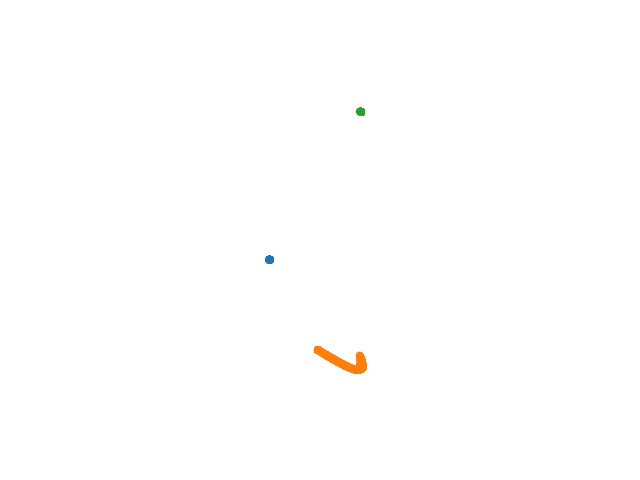
\includegraphics[width=0.3\textwidth]{Figures/odot_graph_spectral.png}

\includegraphics[width=0.3\textwidth]{Figures/odot_graph_result.png}
\caption{\label{fig:graph.laplacian} Example of data transformed using the eigenvectors of the graph Laplacian. Left: Original data. Center: Result of a Kmeans algorithm with three clusters applied to the transformed data (2D projection). Right: Visualization of the cluster labels on the original data.  }
\end{figure}


\section{Deciding the number of clusters}

\subsection{Detecting elbows}
The number, $p$, of subsets with respect to which the population should be partitioned is rarely known a priori, and several methods have been introduced in the literature in order to assess the ideal number of clusters. We now review some of these methods, and denote, for this purpose, by
$\CL^*(p)$ the minimized cost function obtained with $p$ clusters, e.g., using \cref{eq:kmed.2},
\[
\CL^*(p) = \min\{\mW_\al(A_1, \ldots, A_p, c_1, \ldots, c_p): A_1, \ldots, A_p \text{ partition of } T, c_1, \ldots, c_p\in \CR\},
\]
in the case of K-medoids (this definition is algorithm dependent).
It is clear that $\CL^*$ is a decreasing function of $p$. It is also natural to expect that $\CL^*$ should decrease significantly when $p$ is smaller than the correct number of clusters, while the variation should be more marginal when $p$ is overestimated, because the cost in putting together two sets of points that are far apart (which happens when $p$ is too small) is typically larger than the gain in splitting a homogeneous region in two.

The simplest approach in this context is to visualize $\CL^*(p)$ as a function of $p$ and try to locate at which value the resulting curve makes an ``elbow,'' i.e., switches from a sharply decreasing slope to a milder one. \Cref{fig:clusters.elbow} provides an illustration of this visualization when the true number of clusters is three (the data in each cluster following a normal distribution). When the clusters are well separated, an elbow clearly appears on the graph of $\Ga_\al^*$, but this situation is harder to observe when  clusters overlap with each other.
\begin{figure}[h]
\centering
\includegraphics[width=0.4\textwidth]{Figures/ClusterMoG0p25.png}
\includegraphics[width=0.4\textwidth]{Figures/ClusterMoG0p25_inertia.png}\\
\includegraphics[width=0.4\textwidth]{Figures/ClusterMoG0p5.png}
\includegraphics[width=0.4\textwidth]{Figures/ClusterMoG0p5_inertia.png}
\caption{\label{fig:clusters.elbow} Elbow graphs for K-means clustering for two populations generated as mixtures of Gaussian.}
\end{figure}

One can measure the ``curvature'' at the elbow using the distance between each point in the graph of $(p, W_\al^*(p))$ and 
the line between its predecessor and successor. The result gives the criterion
\[
C(p) = \frac{\CL^*(p+1) + \CL^*(p-1) - 2 \CL^*(p)}{\sqrt{(\CL^*(p+1) - \CL^*(p-1))^2 + 4}},
\]
specifying the elbow point as the value of  $p$ at  which $C$ attains its maximum. For both examples in \cref{fig:clusters.elbow}, this method returns the correct number of clusters (3). 


\subsection{The Cali\'nski and Harabasz index}
Several other criteria have been introduced in the literature. \citet{calinski1974dendrite}  propose to minimize the ratio of normalized between-group and within-groups sums of squares associated with K-means. For a given $p$, let $c_1, \ldots, c_p$ denote the optimal centers, and $A_1, \ldots, A_p$ the optimal partition, with $N_k = |A_k|$. The normalized between-group sum of squares is 
\[
h_\al(p) = \frac1{p-1} \sum_{k=1}^p N_k |c_k - \bx|^2
\]
and the normalized within-group sum of squares is   
\[
w_\al(p) = \frac1{N-p} \sum_{k=1}^p \sum_{x\in A_k} |x - c_k|^2
\]
\citet{calinski1974dendrite} suggest to maximize $\ga_{CH}(p) = h_\al(p)/w_\al(p)$. 

This criterion can be extended to other types of cluster analysis. We have seen in \cref{sec:min.disp} that, when $\al(x,y) = |x-y|^2$,
\[
\frac12 \sum_{k=1}^p \sum_{x,y\in A_k} \al(x,y)/N_k = \sum_{k=1}^p \sum_{x\in A_k} |x - c_k|^2.
\]
We also have
\[
\sum_{x\in T} |x-\bx|^2 = \sum_{k=1}^p \sum_{x\in A_k} |x - c_k|^2 + \sum_{k=1}^p N_k |c_k - \bx|^2
\]
and the left-hand side is also equal to 
\[
\frac1{2N} \sum_{x,y\in T} \al(x,y).
\]
It follows that, when  $\al(x,y) = |x-y|^2$,
\[
h_\al(p) =  \frac1{2(p-1)} \left(\frac1N \sum_{x,y\in T} \al(x,y) - \sum_{k=1}^p \sum_{x,y\in A_k} \al(x,y)/N_k\right)
\]
and 
\[
w_\al(p) = \frac1{2(N-p)} \sum_{k=1}^p \sum_{x,y\in A_k} \al(x,y)/N_k.
\]
These expressions can obviously be applied to any dissimilarity measure, extending $\gamma_{CH}$ to general clustering problems. 

\subsection{The ``silhouette'' index}
%Let us introduce some notation, which will lead us to the ``silhouette index'' described in \cite{rousseeuw1987silhouettes}. 
For $x\in T$, let 
\[
d_\al(x, A_k) = \frac1{N_k} \sum_{y\in A_k} \al(x,y).
\]
Let $a_\al(x, p) = d_\al(x, A(x))$ and $b(x, p) = \min\{d_\al(x, A_k): A_k\neq A(x)\}$. Define the  silhouette index of $x$ in the segmentation \citep{rousseeuw1987silhouettes}by
\[
s_\al(x, p) = \frac{b_\al(x,p) - a_\al(x,p)}{\max(b_\al(x,p), a_\al(x,p))} \in [-1,1].
\]
This index measures how well $x$ is classified in the partitioning. It is large when the mean distance between $x$ and other objects in its class is small compared to the minimum mean distance between $x$ and any other class. In order to estimate the best number of clusters with this criterion, one then can maximize the average index:
\[
\ga_{R}(p) = \frac1N \sum_{x\in T} s_\al(x,p).
\]
 
\begin{remark}
One can rewrite the Cali\'nski and Harabasz index using the notation introduced for the silhouette index.
Indeed, let $A(x)$ be the cluster $A_k$ to which $x$ belongs. Then 
\[
h_{\al}(p) =\frac1{2(p-1)} \sum_{x\in T} \sum_{k=1}^p \frac{N_k}{N} (d_\al(x, A_k) - d_\al(x, A(x)))
\] 
and
\[
w_\al(p) = \frac1{2(N-p)} \sum_{k=1}^p \sum_{x\in A_k} d_\al(x, A_k).
\]
\end{remark}
 
\subsection{Comparing to homogeneous data} 
Several selection methods choose $p$ based on the comparison of the data to a ``null hypothesis'' of no cluster. 
For example, assume that K-means is applied to a training set $T$ where samples are drawn uniformly according to the uniform distribution on $[0,1]^d$. Given  centers, $c_1, \ldots, c_p$, let $\bar A_k$ be the set of points in $[0,1]^d$ that are closer to $c_k$ than to any other point. Then the segmentation of $T$ is formed by the sets $A_k = \{x\in T: x\in \bar A_k\}$ and, for large enough $N$, we can approximate $|A_k|/N$ (by the Law of Large Numbers) by the volume of the set $\bar A_k$, that we will denote by $\vol(\bar A_k)$.


\begin{figure}
\centering
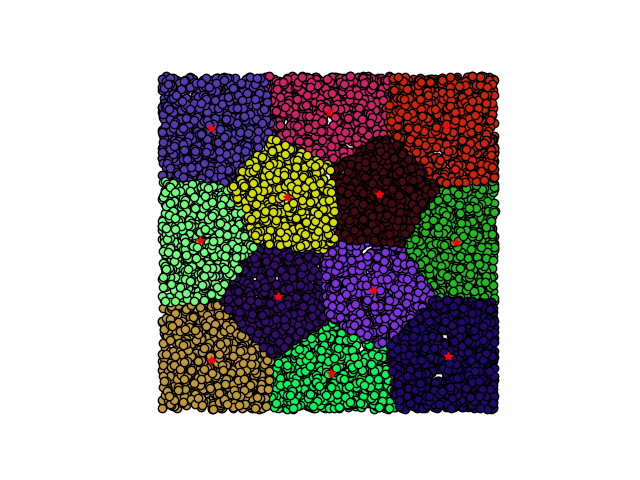
\includegraphics[width=0.75\textwidth]{Figures/uniformCluster.png}
\caption{\label{fig:unif.clust} Division of the unit square into clusters for uniformly distributed data.}
\end{figure}

Let us assume that $c_1, \ldots, c_p$ are uniformly spaced, so that the sets $\bar A_k$ have similar volumes (close to $1/p$) and have roughly spherical shapes (see \cref{fig:unif.clust}). This implies that
\[
\int_{\bar A_k} |x- c_k|^2 dx \simeq \vol(A_k) \frac{r_p^2d}{d+2}
\]
where $r_p$ is the radius of a sphere of volume $1/p$, i.e., $pr_p^d \simeq d/\Gamma_{d-1}$ where $\Gamma_{d-1}$ is the surface area of the unit sphere in $\mR^d$. So, we should have, for some constant $C$ that only depends on $d$,
\[
\sum_{x\in A_k} |x-c_k|^2 \simeq N_k \int_{\bar A_k} |x- c_k|^2 dx  \simeq C(d) (pN)  p^{-2/d-1} = C(d) N p^{-2/d}.
\]
This suggests that, for fixed $N$ and $d$, $p^{2/d} \CL^*(p)$ should vary slowly when $p$ overestimate the number of clusters (assuming that this operation divides an homogeneous cluster). Based on this analysis, \citet{krzanowski1988criterion} introduced the difference-ratio criterion, namely,
\[
\ga_{KL}(p) = \left|\frac{(p-1)^{\frac{2}{d}} \CL^*(p-1) - p^{\frac{2}{d}} \CL^*(p)}{p^{\frac{2}{d}} \CL^*(p) - (p+1)^{\frac{2}{d}} \CL^*(p+1)}\right|,
\]
and estimate the  number of clusters by taking $p$ maximizing $\ga_{KL}$.
\bigskip

Another similar approach, introduced by \citet{sugar2003finding}, is based on an analysis of mixtures of Gaussian, namely assuming an underlying model with $p_0$ groups, where data in group $k$ follow a Gaussian distribution $\CN(\mu_k, \Id)$ (possibly after standardizing the covariance matrix). In that work, the authors show that, if $d$ (the dimension) tends to infinity, with the minimal distance between centers growing proportionally to $\sqrt{d}$, then $\CL^*(p)/d$ tends to infinity when $p < p_0$. They also show that, with similar assumptions, $\CL^*(p)/d$ behaves like $p^{-2/d}$ for $p\geq p_0$, still for large dimensions. Based on this, they suggest using the criterion
\[
\ga_{SJ}(p) = \left(\frac{\CL^*(p)}{d}\right)^{-\nu} - \left(\frac{\CL^*(p-1)}{d}\right)^{-\nu}
\]
(with the convention that $\CL^*(0) = 0$) for some positive number $\nu$ and select the value of $p$ that maximizes $\ga_{SJ}$. Indeed, in the case of Gaussian mixtures, the choice $\nu = d/2$ ensures that, in large dimensions,  $\ga_{SJ}(p)$ is small for $p<p_0$, that it is close to 1 for $p>p_0$ and close to $p_0$ for $p=p_0$.

\bigskip
A more computational approach, based on Monte-Carlo simulations has been introduced in \citet{tibshirani2001estimating}, defining the {\em gap index}
\[
\ga_{TWH}(p)  =  E(\CL^*(p, \mT^\sharp)) - \CL^*(p, T)
\]
where the $\CL^*(p, T)$ denotes the optimal value of the optimized cost with $p$ clusters for a training set $T$. The notation 
$\mT^\sharp$ represent a random training set, with same size and dimension as $T$, generated using an unclustered probability distribution used as a reference.
In \citet{tibshirani2001estimating}, this distribution is taken as uniform (over the smallest hypercube containing the observed data), or uniform on the coefficients of a principal component decomposition of the data (see \cref{chap:dim.red}). The expectation $ E(\CL^*(p, \mT^\sharp))$ is computed by Monte-Carlo simulation, by sampling many realizations of the training set $\mT$, running the clustering algorithm for each of them and averaging the optimal costs.  

One can expect $\CL^*(p, T)$ (for observed data) to decrease much faster (when adding a cluster) than its expectation for homogeneous data when $p<p_0$, and the decrease of both terms to be comparable when $p\geq p_0$. 
 So the number of clusters can in principle be estimated by detecting an elbow in the graph of  $\ga_{TWH}(p)$ as a function of $p$. The procedure suggested in \citet{tibshirani2001estimating} in order to detect this elbow if to look for the first index $p$ such that
\[
\ga_{TWH}(p+1) \leq \ga_{TWH}(p) + \sig(p+1)
\]
where $\sig(p+1)$ is the standard deviation of $\CL^*(p+1, \mT^\sharp)$ for homogeneous data, also estimated via Monte-Carlo simulation. 
\bigskip

Figures \crefrange{fig:clust.indx.1}{fig:clust.indx.3} provide a comparative illustration of some of these indexes.
 \begin{figure}
 \centering
\includegraphics[width=\textwidth]{Figures/MoGIndicesData1.png}
\includegraphics[width=\textwidth]{Figures/MoGIndices1.png}
\caption{\label{fig:clust.indx.1} Comparison of cluster indices for Gaussian clusters. First row: original data and ground truth. Second panel: plots of four indices as functions of $p$ (Elbow; Cali\'nski and Harabasz; silhouette; Sugar and James)}
\end{figure}

 \begin{figure}
 \centering
\includegraphics[width=\textwidth]{Figures/MoGIndicesData2.png}
\includegraphics[width=\textwidth]{Figures/MoGIndices2.png}
\caption{\label{fig:clust.indx.2} Comparison of cluster indices for Gaussian clusters. First row: original data and ground truth. Second panel: plots of four indices as functions of $p$ (Elbow; Cali\'nski and Harabasz; silhouette; Sugar and James).}
\end{figure}

 \begin{figure}
 \centering
\includegraphics[width=\textwidth]{Figures/MoGIndicesData3.png}
\includegraphics[width=\textwidth]{Figures/MoGIndices3.png}
\caption{\label{fig:clust.indx.3} Comparison of cluster indices for Gaussian clusters. First row: original data and ground truth. Second panel: plots of four indices as functions of $p$ (Elbow; Cali\'nski and Harabasz; silhouette; Sugar and James).}

 \end{figure}


\section{Bayesian Clustering}

\subsection{Introduction}
We have seen an example of model-based clustering with mixtures of Gaussian distributions. The main parameters in this model were the number of classes, $p$, and the probabilities $\al_j$ associated to each cluster,  and the parameter of the conditional distribution (e.g., $\CN(c_j, \sig^2\Id_{\mR^d})$) of $X$  conditionally to being in the $j$th cluster. In the approach we described, these parameters were estimated from data using maximum likelihood (through the EM algorithm) and probabilities $f_Z(j|x)$ were then estimated in order to compute the most likely clustering.We interpreted $f_Z(j|x)$  as the conditional probability $P(Z=z|X=x)$, where $Z\in \{1, \ldots, p\}$ represents the group variable. The natural generative order is $Z \to X$: first decide to which group the observation belongs to, then sample the value of $X$ conditional to this group. Clustering is in this case reversing the order, i.e., computing the posterior distribution of $Z$ given $X$.

In a Bayesian approach, the parameters $p, \usal, \usc$ and $\sig^2$ are also considered as random variables, so that  (letting $\underline \th$ denote the vector formed by these parameters), the generative random sequence becomes $\underline{\th} \to Z \to X$. Importantly, $\underline \th$ is assumed to be generated once for all, even if several samples of $X$ are observed, yielding the generative sequence for an $N$-sample,
\[
\underline{\th} \to (Z_1, \ldots, Z_N) \to (X_1, \ldots, X_N).
\]
We use below underlined letters to denote configurations of points, $\usZ = (Z_1, \ldots, Z_N)$, $\usX = (X_1, \ldots, X_N)$, etc. We also use capital letters or boldface letters (for Greek symbols) to differentiate random variable from realizations.

Clusters are still evaluated based on the conditional distribution of $\usZ$ given $\usX$, but this distribution must be evaluated by averaging the conditional distribution of $\usZ$ and $\underline\theta$ given $\usX$ with respect to $\underline \th$, formally\footnote{The symbol $\propto$ means ``equal up to a multiplicative constant''.},
\begin{align*}
P(\usz|\usx) &= \int P(\usz, \underline\th|\usx) P(\underline\th) d\underline\th\\
 &\propto \int \prod_{k=1}^N P(x_k|z_k, \underline\th) P(z_k|\underline\th) P(\underline\th)d\underline\th.
\end{align*}
In this expression, $P(\underline\th)d\underline\th$ implies an integration with respect to the prior distribution of the parameters. This distribution is part of the design of the method, but one usually chooses it so that it leads to simple computations, using so-called {\em conjugate priors}, which are such that posterior distributions belong to the same parametric family as the prior.  For example, the conjugate prior for the mean of a Gaussian distribution (such as $c_i$ in our model) is also a Gaussian distribution. The conjugate prior for a  scalar variance is the inverse gamma distribution, with density  
\[
\frac{v^u}{\Gamma(u)} s^{-u-1}\exp(-v/s)
\]
for some parameters $u,v$. A conjugate prior for the class probabilities $\underline \alpha = (\al_1, \ldots, \al_p)$ is the Dirichlet distribution, with density
\[
D(\al_1, \ldots, \al_p) = \frac{\Gamma(a_1+\cdots + a_p)}{\Ga(a_1) \cdots \Ga(a_p)} \prod_{j=1}^p \al_j^{a_j-1}
\]
on the simplex 
\[
\mathfrak S_p = \{(\al_1, \ldots, \al_p)\in \mR^p: \al_i \geq 0, \al_1+\cdots+\al_p=1\}.
\]


Note that these conjugate priors have the same form (up to normalization) as the parametric model densities when considered as functions of the parameters. 

\subsection{Model with a bounded number of clusters}
We first discuss the Bayesian approach assuming that the number of clusters is smaller than a fixed number, $p$. 
%Alternatively, the joint distribution of $\al_1, \ldots, \al_p$ is that of $\ze_i/(\ze_1 + \cdots + \ze_p), i=1, \ldots, p$ where $\ze_1, \ldots, \ze_p$ are independent and follow a Gamma distribution with parameters $(a_i, 1)$ respectively. 
In this example, we assume  that $c_1, \ldots, c_p$ are modeled as independent Gaussian variables $\CN(0, \tau^2 \Id_{\mR^d})$, $\sig^2$ with an inverse gamma distribution with parameters $u$ and $v$ and $(\al_1, \ldots, \al_p)$ using a Dirichlet distribution with parameters $(a, \ldots, a)$. 

\paragraph{Analytical example.}
The joint probability density of $(\usX, \usZ)$ and $\underline{\boldsymbol \th}$ is proportional to
\begin{multline*}
(\sig^2)^{-u-1} e^{-v/\sig^2} e^{-\sum_{j=1}^p |c_j|^2/2\tau^2} \prod_{j=1}^p \al_j^{a-1}\prod_{k=1}^N \frac{e^{-|x_k - c_{z_k}|^2/2\sig^2}}{(\sig^2)^{d/2}} \prod_{k=1}^N \al_{z_k} \\
= (\sig^2)^{-u-dN/2 -1} \exp\left(- (v + \frac12 \sum_{k=1}^N|x_k-c_{z_k}|^2)/\sig^2\right)\prod_{j=1}^p \al_j^{a+N_j-1} . 
\end{multline*}
One can explicitly integrate this last expression with respect to $\sig^2$ and $\underline\alpha$, using the expressions of the normalizing constants in  the inverse gamma and Dirichlet distributions, yielding (after integration and ignoring constant terms)
\begin{multline*}
\frac{\Ga(a+N_1) \cdots \Ga(a+N_p)}{(v + \frac12 \sum_{k=1}^N|x_k-c_{z_k}|^2)^{u+dN/2}} \exp\left(- \sum_{j=1}^p |c_j|^2/2\tau^2\right)\\
= \frac{\Ga(a+N_1) \cdots \Ga(a+N_p)}{(v + \frac12 S_w + \frac12 \sum_{j=1}^p N_j |c_{j} - \bar x_j|^2)^{u+dN/2}} \exp\left(- \sum_{j=1}^p |c_j|^2/2\tau^2\right)
\end{multline*}
where $S_w = \sum_{k=1}^N |x_k - \bar x_{z_k}|^2$ is the within group sum of squares. Note that this sum of squares depends on $\usx$ and $\usz$, and that $(N_1, \ldots, N_p)$, the group sizes, depend on $\usz$. 

Let us assume a ``non-informative prior'' on the centers, which corresponds to letting $\tau$ tend to infinity and neglecting the last exponential. The remaining expression can now be integrated with respect to $c_1, \ldots, c_p$ by making a change of variables $\mu_j = \sqrt{N_j/(2v+S_k)} (c_j - \bx _j)$ and using the fact that
\begin{multline*}
\int_{(\mR^d)^p} \frac{dc_1\ldots dc_p}{(v + \frac12 S_w + \frac12 \sum_{j=1}^p N_j |c_{j} - \bar x_j|^2)^{u+dN/2}} = \\
(2v+S_w)^{(p-N)d/2 - u)}  \prod_{j=1}^p N_j^{-d/2}\int_{(\mR^d)^p} \frac{d\mu_1\ldots d\mu_p}{(\frac12+ \frac12 \sum_{j=1}^p |\mu_j|^2)^{u+dN/2}}
\end{multline*}
and the final integral does not depend on $\usx$ or  $\usz$. It follows from this that the conditional distribution of $\usZ$ given $\usx$ takes the form
\[
P(\usz|\usx) = C(\usx)\frac{\prod_{j=1}^p \Ga(a+N_j)}{(2v+S_w)^{(N-p)d/2 + u)}  \prod_{j=1}^p N_j^{d/2}}
\]
where $C(\usx)$ is a normalization constant ensuring that the right-hand side is a probability distribution over configurations $\usz = (z_1, \ldots, z_N) \in \{1, \ldots, p\}^N$. In order to obtain the most likely configuration for this posterior distribution, one should therefore minimize in $\usz$ the function
\[
((N-p)\frac d2 +u)\log (2v+S_w) + \frac d2 \sum_{j=1}^p \log N_j  -\sum_{j=1}^p \log \Ga(a+N_j).
\] 
This final optimization problem cannot be solved in closed form, but this can be performed numerically.  One can simplify it a little by only keeping the main order terms in the last two sums (using Stirling formula for the Gamma function) and minimize
\[
((N-p)\frac d2 +u)\log (2v+S_w)  - \sum_{j=1}^p (a+N_j) \log (a+N_j).
\] 
This expression has a nice interpretation, since
the first term minimizes the within-group sum of squares, the same objective function as in K-means, and the second one is an entropy term that favors clusters with similar sizes.

\paragraph{Monte-Carlo simulation.}
An alternative  to this analytical  approach is to use Monte-Carlo simulations to estimate some properties of the posterior distribution numerically. While they are often computationally demanding, Monte-Carlo methods are more flexible and can be used in situations when analytic computations are in\-trac\-table. In order to sample from the distribution of $\usZ$ given $\usx$, it is actually easier to sample from the joint distribution of $(\usZ, \underline{\boldsymbol \th})$ given $\usx$, because this distribution has a simpler form. Of course, if the pair $(\usZ, \underline{\boldsymbol \th})$ is sampled from the conditional distribution given $\usx$, the first component, $\usZ$ will follow the posterior distribution we are interested in. 

In the context of the discussed example, this reduces to sampling from a distribution proportional to 
\begin{equation}
\label{eq:MoG.posterior}
(\sig^2)^{-u-1} e^{-v/\sig^2} e^{-\sum_{j=1}^p |c_j|^2/2\tau^2} \prod_{j=1}^p \al_j^{a-1}\prod_{k=1}^N \frac{e^{-|x_k - c_{z_k}|^2/2\sig^2}}{(\sig^2)^{d/2}} \prod_{k=1}^N \al_{z_k}\,.
\end{equation}
Sampling from all these variables at once is  not tractable, but it is easy to sample from them in sub-groups, conditionally to the rest of the variables. We can, for example, deduce from the expression above the following conditional distributions.
\begin{enumerate}[label=(\roman*), wide=0.5cm]
\item Given $(\underline\alpha, \usc, \usz)$, $\sig^2$ follows an inverse gamma distribution with parameters $u+dN/2$ and $v + \frac12 \sum_{k=1}^N|x_k-c_{z_k}|^2$. 
\item Given $(\usz, \usz, \sig^2)$, $\underline\alpha$ follows a Dirichlet distribution with parameters $a+N_1, \ldots, a+N_p$.
\item Given $(\usz, \sig^2, \underline\alpha)$, $c_1, \ldots, c_p$ are independent and follow a Gaussian distribution, respectively with mean $(1 + \sig^2/(N_j\tau^2))^{-1} \bar x_j$ and variance $(N_j/\sig^2 + 1/\tau^2)^{-1}$.
\item Given $(\sig^2, \underline\alpha, \usc)$, $z_1, \ldots, z_N$ are independent and 
\[
P(z_k=j|\sig^2, \usal, \usc, \usx) \propto \al_j e^{-|x_k-c_j|^2/2\sig^2}.
\]
\end{enumerate}



\begin{algorithm}[Gibbs sampling for mixture of Gaussian (Bayesian case)]
\label{alg:gs.MoG}
\begin{enumerate}[label=(\arabic*)]
\item Initialize with variables $\underline\alpha, \usc, \sig$ and $\usz$, for example generated according to the prior distribution.
\item Loop a large number of times over the following steps.
\begin{enumerate}[label=(\roman*),wide=1cm]
\item Simulate  a new value of $\sig^2$ according to an inverse gamma distribution with parameters $u+dN/2$ and $v + \frac12 \sum_{k=1}^N|x_k-c_{z_k}|^2$. 
\item Simulate new values for $\al_1, \ldots, \al_p$ according to a Dirichlet distribution with parameters $a+N_1, \ldots, a+N_p$.
\item Simulate new values for  $c_1, \ldots, c_p$ independently, sampling $c_i$ according to a Gaussian distribution with mean $(1 + \sig^2/(N_j\tau^2))^{-1} \bar x_j$ and variance $(N_j/\sig^2 + 1/\tau^2)^{-1}$.
\item Simulate new values of $z_1, \ldots, z_N$ independently such that
\[
P(z_k=j|\sig^2,\usal, \usc, \usx) \propto \al_j e^{-|x_k-c_j|^2/2\sig^2}.
\]
\end{enumerate}
\end{enumerate}
\end{algorithm}

Note that this algorithm is only asymptotically providing a sample of the posterior distribution (it has to be stopped at some point, of course). Note also that, at each step, the labels $z_1, \ldots, z_N$ provide a random partition of the set $\{1, \ldots, N\}$, and this partition changes at every step. 

To estimate one single partition out of this simulation, several strategies are possible. Using the simulation, one can estimate the probability $w_{kl}$ that $x_k$ and $x_l$ belong to the same cluster. This can be dome by averaging the number of times that $z_k = z_l$ was observed along the Gibbs sampling iterations (from which one usually excludes a few early ``burn-in'' iterations). These weights, $w_{kl}$ can then be used as similarity measures in a clustering algorithm.

Alternatively, one can average for each $k$, the values of the class center $c_{z_k}$ associated to $k$, still along the Gibbs sampling iterations. These average values can then be used as input of, say, a K-means algorithm to estimate final clusters.

\paragraph{Mean-field approximation.}
We conclude this section with a variational Bayes approximation of the posterior distribution. We will make a mean-field approximation, in which all parameters and latent variables are independent, therefore approximating the distribution in \cref{eq:MoG.posterior} by a product distribution taking the form
\[ g(\sigma^2, \underline\alpha, \underline c, \underline z) = 
g^{(\sigma^2)}(\sigma^2) g^{(\alpha)}(\underline \alpha) \prod_{j=1}^p g^{(c)}_j(c_j)\prod_{k=1}^N g^{(z)}_k(z_k).
\]
Here $\underline c = (c_1, \ldots, c_p)$, $\underline z = (z_1, \ldots, z_N)$ and $\underline\alpha = (\alpha_1, \ldots, \alpha_p)$. We have $\sigma^2 \in (0, +\infty)$, $\underline c \in (\mR^{d})^p$, $\underline\alpha\in \mathcal S$, the set of all non-negative $\al_1, \ldots, \alpha_p$ that sum to one, and $\underline z\in \{1, \ldots, p\}^N$ (so that $g_k^{(x)}$ is a p.m.f. on $\{1, \ldots, p\}$.  We will use the discussion in \cref{sec:mean.field} and \cref{lem:max.ent}, and use the notation introduced in that section to denote as  $\avg{\boldsymbol\phi}$ the expectation a variable $\boldsymbol\varphi$ of the variables above for the p.d.f. $g$.

The log-likelihood for a mixture of Gaussian takes the form (ignoring contant terms)
\begin{align*}
\ell(\sigma^2, \underline \alpha, \underline c, \underline z ) =& 
  -(u+1) \log \sigma^2 - v\sigma^{-2}  
- \frac1{2\tau^2} \sum_{k=1}^p |c_j|^2 + \sum_{j=1}^p (a-1)\log \alpha_j  \\ 
&- \frac{Nd}{2} \log \sigma^2
- \frac12 \sigma^{-2}  \sum_{k=1}^N |x_k-c_{z_k}|^2  + \sum_{k=1}^N \log\alpha_{z_k}\\
= & -(u+1) \log \sigma^2 - v\sigma^{-2} - \frac1{2\tau^2} \sum_{k=1}^p |c_j|^2 + \sum_{k=1}^p (a-1)\log \alpha_j  \\ 
&- \frac{Nd}{2} \log \sigma^2
- \frac12 \sigma^{-2}  \sum_{k=1}^N \sum_{j=1}^p |x_k-c_{j}|^2 \bfone_{z_k=j}  + \sum_{k=1}^N \sum_{j=1}^p \log\alpha_{j} \bfone_{z_j=k}
\end{align*}
and can therefore be decomposed as  a sum of products of functions of single variables, as assumed in \cref{sec:mean.field}. Using \cref{lem:max.ent}, we can identify each of the distributions composing $g$, namely:
\begin{itemize}
\item $g^{(\sigma^2)}$ is the p.d.f. of an inverse gamma with parameters $\tilde u = u+Nd/2$ and
\[
\tilde v = \nu + \frac12   \sum_{k=1}^N \sum_{j=1}^p \avg{|x_k-C_j|^2}\, \avg{Z_k=j}.
\]
\item  $g_j^{(c)}$ is the p.d.f. of a Gaussian, with parameters  $\CN(\tilde m_j, \tilde \sigma_j^2\Id[d])$, with, letting
\[
\tilde \zeta(j) = \sum_{k=1}^N \avg{Z_k=j} = \sum_{k=1}^N g^{(z)}_k(j),
\]
$\tilde \sigma^2_j =  \left(\frac1{\tau^2} + \avg{\boldsymbol\sigma^{-2}} \tilde\zeta(j) \right)^{-1}$ and
$\tilde m_i = \avg{\boldsymbol\sigma^{-2}} \tilde \sigma^2_j  \sum_{k=1}^N \avg{Z_k=j} x_k$.
\item 
 $g^{(\alpha)}$ of a Dirichlet distribution, with parameters $\tilde a_1, \ldots, \tilde a_k$, with $\tilde a_i = a + \tilde \zeta(j) $.
 \item Finally $g_k^{(z)}$ is a p.m.f. on $\{1, \ldots, p\}$ with
 \[
 g_k^{(z)}(j) \propto \exp\left(- \frac12 \avg{\boldsymbol\sigma^{-2}} \avg{|x_k-C_j|^2} +\avg{\log \boldsymbol\alpha_j}\right).
\]
\end{itemize}

To complete the consistency equations, it now suffices to evaluate the expectations in the formula above as functions of the other parameters. We leave to  the reader the verification of the following statements.
\begin{itemize}
\item If $\boldsymbol\sigma^2$ follows an inverse gamma distribution with parameters $\tilde{u}$ and $\tilde{v}$, then  $\avg{\sigma^{-2}} = \tilde{u}/\tilde{v}$.
\item If $C_j \sim \CN(\tilde m_j, \tilde{\sigma}^2_j \Id[d])$, then $\avg{|x_k-C_j|^2} = |x_k-\tilde m_j|^2 + d\tilde{\sigma}^2_j$. 
\item  If $\underline{\boldsymbol\alpha}$ follows a Dirichlet distribution with parameters $\tilde a_1, \ldots, \tilde a_p$, then $\avg{\log\boldsymbol\alpha_j} = \psi(\tilde a_j) - \psi(\tilde a_1+\cdots + \tilde a_p)$ where $\psi$ is the {\em digamma} function (derivative of the logarithm of the gamma function).
\end{itemize}

Combining these facts with the expression of the mean-field parameters, we can now formulate a mean-field estimation algorithm for mixtures of Gaussian that iteratively applies the consistency equations.

\begin{algorithm}[Mean-field algorithm for mixtures of Gaussian]
\label{alg:mean.field.mog}
\begin{enumerate}[label=(\arabic*), wide=0.5cm]
\item: Input: training set $(x_1, \ldots, x_N)$, number of clusters $p$, prior parameters $u, v, \tau^2$ and $a$ .
\item Initialize variables $\tilde \sigma^2_1, \ldots, \tilde \sigma^2_p$, $\tilde m_1, \ldots, \tilde m_p$, $\tilde a_1, \ldots, \tilde a_p$, $\tilde g_k(j)$, $k=1, \ldots, N$, $j=1, \ldots, p$. 
%\item Let $\tilde u = u+Nd/2$.
\item Let  $\tilde \zeta(j) = \sum_{k=1}^N \tilde g_k(j)$, $j=1, \ldots, p$.
\item Let 
\[
\tilde \rho^2 = \frac{1}{u+Nd/2} \left(v + \frac12 \sum_{k=1}^N \sum_{j=1}^p \tilde g_k(j) |x_k-\tilde m_j|^2 + \frac{d}2 \sum_{j=1}^p \tilde\sigma_j^2\tilde\zeta(j)\right).
\]
\item For $j=1, \ldots, p$, let $\tilde \sigma^2_i =  \left(\frac1{\tau^2} +\frac{\tilde\zeta(j)}{\tilde \rho^2} \right)^{-1}$ and $\tilde m_i = \frac{\tilde\sigma_j^2}{\tilde \rho^2} \sum_{k=1}^N \tilde g_k(j) x_k$.
\item Let $\tilde a_i = a + \tilde \zeta(j) $, $j=1, \ldots, p$.
\item For $k=1, \ldots, N$, $j=1, \ldots, p$, let
\[
\tilde g_k(j) \propto \exp\left(- \frac1{2\tilde\rho^2}  \left(|x_k-\tilde m_j|^2 + d \tilde\sigma_j^2\right) + \psi(\tilde a_j) \right).
\]
\item Compare the updated variables with their previous values and stop if the difference is below a tolerance level. Otherwise, return to (3).
\end{enumerate}
\end{algorithm}
After convergence $g_k^{(z)}$ provides the mean-field approximation of the posterior probability of classes for observation $k$ and can be used to determine clusters.

\subsection{Non-parametric priors}
\label{sec:cluster.npb}
\paragraph{The Polya urn}
In the previous model with $p$ clusters or less, the joint distribution of $Z_1, \ldots, Z_N$ is given by
\[
\pi(z_1, \ldots, z_N) = \frac{\Ga(pa)}{\Ga(a)^p} \int_{\mathfrak S_p} \prod_{j=1}^p \al_j^{a+N_j -1} d\al = \frac{\Ga(pa)}{\Ga(pa+N)} \prod_{j=1}^p \frac{\Ga(a+N_j)}{\Ga(a)}.
\]
Conditional to $z_1, \ldots, z_N$, the data model was completed by sampling $p$ sets of parameters, say, $\th_1, \ldots, \th_p$, each belonging to a parameter space $\Th$  and following a prior probability distribution with density, say, $\psi$ and variables $X_1, \ldots, X_N$, where $X_k\in \CR$ was drawn according to a law dependent on its cluster, that we will denote $\phi(\,\cdot\mid\th_{z_k})$. The complete likelihood of the data is now
\[
L(\usz, \underline\th, \usx) = \frac{\Ga(pa)}{\Ga(pa+N)} \prod_{j=1}^p \frac{\Ga(a+N_j)}{\Ga(a)} \prod_{j=1}^p \psi(\th_j) \prod_{k=1}^N \phi(x_k|\th_{z_k}).
\]


Note that the right-hand side does not change if one relabels the values of $z_1, \ldots, z_N$, i.e., if one replaces each $z_k$ by $s(z_k)$ where $s$ is a permutation of $\{1, \ldots, p\}$, creating a new configuration denoted $s\cdot \usz$. Let $[\usz]$ denote the equivalence class of $\usz$, containing all $\usz' = s \cdot \usz, s\in \mathfrak S_N$: all the labelings in $[\usz]$ provide the same partition of $\{1, \ldots, N\}$ and can therefore be identified. One defines a probability distribution $\bar\pi$ over these equivalence classes by letting
\[
\bar \pi([\usz]) = |[\usz]|\frac{\Ga(pa)}{\Ga(pa+N)} \prod_{j=1}^p \frac{\Ga(a+N_j)}{\Ga(a)}.
\]
The first term on the right-hand side is  the number of elements in the equivalence class of $[\usz]$. To compute it, 
let $p_0 = p_0(\usz)$ denote the number of different values  taken by $z_1, \ldots, z_N$, i.e., the ``true'' number of  clusters (ignoring the empty ones), which now is a function of $\usz$. Let $A_1, \ldots, A_{p_0}$ denote the partition associated with $\usz$.  New labelings equivalent to $\usz$ can be obtained by assigning any index $i_1\in \{1, \ldots, p\}$ to elements of $A_1$, then any index $i_2\neq i_1$ to elements of $A_2$, etc., so that there are  $|[\usz]| = p!/(p-p_0)!$ choices. We therefore find:
\[
\bar \pi([\usz]) = \frac{p!}{(p-p_0)!} \frac{\Ga(pa)}{\Ga(pa+N)} \prod_{j=1}^p \frac{\Ga(a+N_j)}{\Ga(a)}.
\]
Letting $\la = pa$ and using the formula $\Ga(x+1) = x\Ga(x)$, this can be rewritten as
\[
\bar \pi([\usz]) = \frac{p(p-1)\cdots(p-p_0+1)}{\la (\la+1) \ldots (\la+N-1)} \prod_{j=1}^p \prod_{i=0}^{N_j-1} (\la/p+i).
\]

Now, the class $[\usz]$ contains exactly one element $\hat \usz$ with the following properties
\begin{enumerate}[label=$\bullet$, wide=0.5cm]
\item $\hat z_1 = 1$,
\item $\hat z_k \leq \max(z_j, j<k) + 1$ for all $k>1$.
\end{enumerate}
This means that the $k$th label is either one of those already appearing in $(\hat z_1, \ldots, \hat z_{k-1})$ or the next integer in the enumeration. We will call such a $\hat \usz$ admissible. % and let $\CZ_N$ denote the set of such admissible labelings. 
If we assume that $\usz$ is admissible in the expression of $\bar \pi$, we can write
\[
\bar \pi([\usz]) = \frac{\prod_{j=1}^{p_0} \left(\la (1-j/p) \prod_{i=1}^{N_j-1} (\la/p + i)\right)}{\la (\la+1) \ldots (\la+N-1)}.
\]
If one takes the limit $p\to\infty$ in this expression, one still gets a probability distribution on admissible labelings, namely
\begin{equation}
\label{eq:dp.classes}
\bar \pi([\usz]) = \frac{\la^{p_0} \prod_{j=1}^{p_0} (N_j-1)! }{\la (\la+1) \ldots (\la+N-1)}.
\end{equation}
Recall that, in this equation, $p_0$ is a function of $\usz$, equal, for admissible labelings, to the largest $j$ such that $N_j > 0$.


The probability $\bar \pi$ is generated by the following sampling scheme, called the Polya urn process simulating admissible labelings.

\begin{algorithm}[Polya Urn]
\label{alg:polya.urn}
\begin{enumerate}[label=\arabic*, wide=0.5cm]
\item Initialize $k=1$, $z_1=1$, $j=1$. Let $N_1 = 1$
\item At step $k$, assume that $z_1, \ldots,  z_k$ have been generated, with associated number of clusters equal to $j$ and $N_1, \dots, N_j$ elements per cluster. Generate $z_{k+1}$ such that
\begin{equation}
\label{eq:polya.urn}
z_{k+1} = 
\left\{
\begin{aligned}
&i&& \text{ with probability } && \frac{N_i}{\la + k}, \text{ for } i=1, \ldots, j\\
&j+1&& \text{ with probability } && \frac{\la}{\la + k}
\end{aligned}
\right.
\end{equation}
\item If $z_{k+1} = i \leq j$, then replace $N_i$ by $N_{i}+1$, $k$ by $k+1$.
\item If $z_{k+1} = j+1$, let $N_{j+1} = 1$, replace $j$ by $j+1$ and $k$ by $k+1$.
\item If $k<N$, return to step 2, otherwise, stop.
\end{enumerate}
\end{algorithm}
%If $z_1, \ldots, z_N$ are generated according to this algorithm, then

Using this prior, the complete model for the distribution of the observed data is
\[
L(\usz, \underline \th, \usx) = \frac{\la^{p_0} \prod_{j=1}^{p_0} (N_j-1)! }{\la (\la+1) \ldots (\la+N-1)} \prod_{j=1}^{p_0} \psi(\th_j) \prod_{k=1}^N \phi(x_k|\th_{z_k})
\]
Recall that, in this expression, $\usz$ is restricted to the set of admissible labelings. We also note that admissible labelings are in one-to-one correspondence with the partitions of $\{1, \ldots, N\}$, so that the latent variable $\usz$ in this expression can also be interpreted as representing a random partition of this set. 


\paragraph{Dirichlet processes.}

As we will see later, the expression of the global likelihood and the Polya urn model will suffice for us to develop  non-parametric clustering methods for a set of observations  $x_1, \ldots, x_N$. However, this model is also associated to an important class of random probability distributions (i.e., random variables taking values in some set of probability distributions) called Dirichlet processes for which we provide a brief description.

The distribution in \cref{eq:dp.classes} was obtained by passing to the limit from a  model 
that first generates $p$ numbers $\al_1, \ldots, \al_p$, then generates the labels $z_1, \ldots, z_N \in \{1, \ldots, p\}$ identified modulo relabeling. This distribution  can also be defined directly, by first defining an infinity of positive numbers $(\al_j, j\geq 1)$ such that $\sum_{i=1}^\infty \al_i = 1$,  followed by the generation of random labels $Z_1, \ldots, Z_N$ such that $P(Z_k = j) = \al_j$, followed once again with an identification up to relabeling.

 The distribution of $\underline{\boldsymbol \al}$ that leads to the Polya urn is called the {\em stick breaking process}. This process is such that
\[
\bfal_j = U_j \prod_{i=1}^{j-1}(1-U_i)
\] 
where $U_1, U_2, \ldots$ is a sequence of i.i.d. variables following a $\mathrm{Beta}(1, \la)$ distribution, i.e., with p.d.f. $\la (1-u)^{\la-1}$ for $u\in [0,1]$. The stick breaking interpretation comes from the way $\bfal_1, \bfal_2, \ldots$ can be simulated: let $\bfal_1 \sim \mathrm{Beta}(1, \la)$; given $\bfal_1, \ldots, \bfal_{j-1}$, let $\bfal_j = (1-\bfal_1 - \cdots - \bfal_{j-1})U_j $ where $U_j \sim \mathrm{Beta}(1, \la)$ and is independent from the past. Each step can be thought of as breaking the remaining length, $(1-\bfal_1 - \cdots - \bfal_{j-1})$, of an original stick of length 1 using a beta-distributed variable, $U_j$. This process leads to the distribution \cref{eq:dp.classes} over admissible distributions, i.e., if $\al$ is generated according to the stick breaking process, and $Z_1, \ldots, Z_N$ are independent, each such that $P(Z_k=j) = \al_j$, then the probability that $(Z_1, \ldots, Z_N)$ is identical, after relabeling, to the admissible configuration $z$ is given by \cref{eq:dp.classes}. (We skip the proof of this result, which is not straightforward.)



Now, take a realization $\usal = (\al_1, \al_2, \ldots)$ of the stick-breaking process, and independent realizations $\useta = (\eta_1,  \eta_1, \ldots)$ drawn according to the p.d.f. $\psi$. Define
\begin{equation}
\label{eq:dir.proc}
\rho = \sum_{j=1}^\infty \al_j \de_{\eta_j}\,.
\end{equation}
For any realization of $\bfal$ and of $\bfeta$, $\rho$ is a probability distribution on the parameter space $\Th$ (in which one chooses $\eta_i$ with probability $\al_i$). Since $\bfal$ and $\bfeta$ are both random variables, this defines a random variable $\boldsymbol\rho$  with values in the space of probability measures on $\Th$.


This process has the following characteristic property. For any family $V_1, \ldots, V_k\sub \Th$ forming a partition of that set,  the random variable $(\boldsymbol\rho(U_1), \ldots, \boldsymbol\rho(U_k))$  follows a Dirichlet distribution with parameters 
\[
\left(\la \int_{U_1} \psi\,d\eta , \ldots, \la \int_{U_1} \psi\,d\eta \right).
\] 
This is the definition of  a Dirichlet process with parameters $(\la, \psi)$, or, simply, with parameter $\la\psi$. Conversely, one can also show that any Dirichlet process can be decomposed as in \cref{eq:dir.proc} where $\bfal$ is a stick-breaking process and $\bfeta$ independent realizations of $\psi$.

% and a common choice is to use a generalization of the Dirichlet distribution that was used for finite $p$, called the Dirichlet process. To motivate the definition, we note that if $\al_1, \ldots, \al_p$ follow a Dirichlet distribution with parameters $a_1, \ldots, a_p$, then 
%$\al_1$ follows a  beta distribution with parameters $(a_1, a_2+\cdots+a_p)$. Moreover, conditionally to $\al_1$, the variables $(\al_j/(1-\al_1), j>1)$ follow a Dirichlet distribution with parameters $(a_{2}, \ldots, a_p)$. 

%%The simulation of the i.i.d. variables describing a cluster decomposition according to this process $(\eta_1, \ldots, \eta_N)$ would in principle require simulating the stick-breaking process and the parameters $\eta^{(1)}, \eta^{(2)}, \ldots$ first, then, for all $k=1, \ldots, N$, sample $\eta_k = \eta^{(j)}$ with probability $\al_j$. 
%%An interesting feature of the Dirichlet process is that one can simulate $(\eta_1, \ldots, \eta_N)$ directly through another random process called the Polya Urn. This process is initialized by sampling $\eta^{(1)}$ at random according to $\psi$ and letting $z_1 = 1$.
%%
%%Assume that, after step $k$, $p$ values $\eta^{(1)}, \ldots, \eta^{(p)}$ have been obtained and variables $z_1, \ldots, z_k$ have been determined, all taking values in $\{1, \ldots, p\}$. Let $N_i$ denote the number of indices $l$ such that $z_l = i$. 
%%One then samples $z_{k+1} \in \{1, \ldots, p+1\}$ according to the following probabilities
%%\[
%%P(z_{k+1} = i|z_1, \ldots, z_k) = \left\{
%% \begin{aligned}
%%\frac{N_i}{\la + k} &\text{ if } i \leq p \\
%%\frac{\la}{\la+k} & \text{ if } i = p+1
%%\end{aligned}
%%\right.
%%\]
%%If $z_{k+1} = p+1$, sample a new value $\eta^{(p+1)}$ and replace $j$ by $p+1$ for the next step.
%%
%%When $k=N$, set $\eta_l = \eta^{(z_l)}$ for $l=1, \ldots, N$. One can also write in closed form the joint distribution of the class variables $(z_1, \ldots, z_N)$, namely: $z_1 = 1$ and 
%%\begin{equation}
%%P(z_2, \ldots, z_N) = \frac{\la^{p-1} \prod_{j=1}^p (N_j-1)!}{(\la+1) \cdots (\la+N-1)}.
%%\end{equation}
%%Note that in this formula, $p, N_1, \ldots, N_p$ are all functions of $z_2, \ldots, z_N$. This probability is supported on admissible configurations, where  $z_1, \ldots, z_N$ is admissible if and only if $z_1=1$ and $z_k \leq \max(z_j, j<k) + 1$ for all $k>1$. For such a configuration, we have $p = \max(z_1, \ldots, z_N)$.
%%
%Of course, we can also express the stick-breaking process uniquely in terms of the parameters $\eta^{(1)}, \ldots, \eta^{(p)}$ and their assignments to observations, $\eta_1, \ldots, \eta_N$. Indeed, let $\eta^{(1)} \sim \psi$ and $\eta_1 = \eta^{(1)}$.
%
%Assume that $\eta_1, \ldots, \eta_k$ have been sampled, and let $\eta^{(1)}, \ldots, \eta^{(p_k)}$ denote the distinct values in  $\eta_1, \ldots, \eta_k$ listed in order of appearance. Let $N^{(k)}_j$ denote the number of indices $l\leq k$ such that $\eta_l = \eta^{(j)}$.
%Then, the next variable $\eta_{k+1}$ is obtained by:
%\begin{enumerate}
%\item Sampling a new variable $\eta^{(p_k) + 1}$ according to the distribution $\psi$;
%\item Setting $\eta_{k+1} = \eta^{(j)}$ with  probability $N_j^{(k)}/(\la+k)$ with probability if $j \leq p_k$ and $\la/(\la+k)$ if $j=p_k+1$.
%\end{enumerate}
%
%Importantly, the right-hand term  in \eqref{eq:dp.classes} is permutation-invariant in the following sense. If $S$ is a permutation of $\{1, \ldots, N\}$, let $S\cdot(z_1, \ldots, z_N) = (z'_1, \ldots, z'_N)$ where $z'_1, \ldots, z'_N$ is computed as follows:
%\begin{enumerate}
%\item Reorder $z_1, \ldots, z_N$ as $z_{S(1)}, \ldots, z_{S(N)}$. 
%\item Relabel the reordered sequence to make it admissible, namely let $z'_1 = i$ and, for $k]>1$, let $z'_k = z'_j$ if there  exists $j< k$ such that $z_{S(j)} = z_{S(k)}$ and equal to $\max(z'_j, j<k)+1$ otherwise.
%\end{enumerate}
%
%This shows that the conditional probability of $z_k = i$ given $z_l, l\neq k$ can be deduced form the final step of the stick breaking process after applying the permutation that moves $z_k$ to the last place while keeping the order of the other variables unchanged. Let $S^{(k)}$ denote this permutation, and $( z'_{1,k}, \ldots, z'_{N,k}) = S^{(k)}\cdot (z_1, \ldots, z_N)$. Let $p^-_k$ be the number of distinct values in $z'_{l,k},  l< N$, and $N^-_{i,k}$ the number of times $z'_{l,k} = 1$ among the same variables, for $i\leq p^-_k$.
%Then, 
%\begin{equation}
%\label{eq:stick.cond}
%P(z'_{N,k} = i|z'_{l,k} l\neq k) = \left\{
% \begin{aligned}
%\frac{N^-_{i,k}}{\la + N-1} &\text{ if } i \leq p^-_k \\
%\frac{\la}{\la+N-1} & \text{ if } i = p^-_k+1
%\end{aligned}
%\right.
%\end{equation}


\paragraph{Monte-Carlo simulation.}
The joint distribution of labels, parameters and observed variables can also be deduced from \cref{eq:dp.classes}, with a joint p.d.f. given by
\begin{equation}
\label{eq:dp.mix}
\frac{\la^{p_0-1} \prod_{j=1}^{p_0} (N_j-1)!}{(\la+1) \cdots (\la+N-1)} \prod_{j=1}^{p_0} \psi(\eta_j) \prod_{k=1}^N \phi(x_k|\eta_{z_k}).
\end{equation}
The forward simulation of this distribution is a straightforward extension of \cref{alg:polya.urn}, namely:
\begin{algorithm}
\label{alg:polya.urn.complete}
\begin{enumerate}[label=\arabic*, wide=0.5cm]
\item Initialize $k=1$, $z_1=1$, $j=1$. Let $N_1 = 1$.
\item Sample $\eta_1\sim \psi$ and $x_1 \sim \phi(\cdot|\eta_1)$.
\item At step $k$, assume that $z_1, \ldots,  z_k$ has been generated, with associated number of clusters equal to $j$ and $N_1, \dots, N_j$ elements per cluster. Generate $z_{k+1}$ such that
\[
z_{k+1} = 
\left\{
\begin{aligned}
&i&& \text{ with probability } && \frac{N_i}{\la + k}, \text{ for } i=1, \ldots, j\\
&j+1&& \text{ with probability } && \frac{\la}{\la + k}
\end{aligned}
\right.
\]
\item If $z_{k+1} = i \leq j$, sample $x_{k+1} \sim \phi(\,\cdot\, | \eta_i)$. Replace $N_i$ by $N_{i}+1$, $k$ by $k+1$.
\item If $z_{k+1} = j+1$, let $N_{j+1} = 1$, sample $\eta_{j+1} \sim \psi$ and $x_{k+1} \sim \phi(\,\cdot\, | \eta_{j+1})$. Replace $j$ by $j+1$ and $k$ by $k+1$.
\item If $k<N$, return to step 2, otherwise, stop.
\end{enumerate}
\end{algorithm}

This algorithm cannot be used, of course, to sample from the conditional distribution of $Z$ and $\bfeta$ given $X=x$, and Markov-chain Monte-Carlo must be used for this purpose.  In order  to describe how Gibbs sampling may be applied to this problem, we  use the fact that, as previously remarked, using admissible labelings $z$ is equivalent to using partitions $\CA = (A_1, \ldots, A_{p_0})$ of $\{1, \ldots, N\}$, and we will use the latter formalism to describe the algorithm. We will also use the notation $\eta_A$ to denote the parameter associated to $A\in \CA$ so our new notation for the variables is $(\CA, \useta)$ where $\CA$ is a partition of $\{1, \ldots, N\}$ and $\useta$ is a collection $(\eta_A, A\in \CA)$ with $\eta_A \in \Th$.
Given this, we want to sample from a conditional p.d.f.
\begin{equation}
\label{eq:dp.mix.cond}
\Phi(\CA, \useta | x) \propto \frac{\la^{|\CA|-1} \prod_{A\in\CA} (|A|-1)!}{(\la+1) \cdots (\la+N-1)} \prod_{A \in \CA} \psi(\eta_A) \prod_{k\in A}  \phi(x_k|\eta_A). 
\end{equation}
As an additional notation, given a partition $\CA$ and an index $k\in \{1. \ldots, N\}$, we let $\CA_k$ denote the set $A$ in $\CA$ that contains $k$.

The following points are relevant for the design of the sampling algorithm. 
\begin{enumerate}[label=(\arabic*), wide=0.5cm]
\item The conditional distribution of $\underline \bfeta$ given $\CA$ and the training data is proportional to 
\[
\prod_{A\in\CA} \left(\psi(\useta_A) \prod_{k\in A}  \phi(x_k|\useta_A)\right) 
\]
This shows that the parameters $\eta_A, A\in \CA$  are independent of each other, with $\eta_A$ following a distribution proportional to
\[
\eta \mapsto \psi(\eta) \prod_{k\in A_j}  \phi(x_k|\eta).
\]
Sampling from this distribution generally offers no special difficulty, especially if the prior $\psi$ is conjugate to $\phi$. Importantly, one does not need to sample exactly from $\eta_A$, and it is often more convenient to separate $\eta_A$ into several components (such as mean and variance for mixtures of Gaussian) and sample from them alternatively, creating another level of Gibbs sampling.


\item We now consider  the issue of updating $\CA$. We will use for this purpose the formalism of \cref{alg:gibbs.sampling}. In particular,  for each $k\in \{1, \ldots, N\}$, we associate to the variable $ (\CA, \useta)$ the pair $(\CA^{(k)}, \useta^{(k)})$, where $\CA^{(k)}$ is the partition  of $\{1, \ldots, N\} \setminus\{k\}$ formed by the sets $A^{(k)}  = A \setminus \{k\}$  and $\eta_A^{(k)} = \eta_A$, unless $A = \{k\}$, in which case the set and the corresponding $\eta_A$ are dropped. 

We can write $\Phi(\CA, \useta|\usx)$ in the form
\begin{equation}
\label{eq:dp.gs.1}
\Phi(\CA, \useta|\usx) \propto q(\CA_k, \eta_{\CA_k}) \phi(x_k|\eta_{\CA_k})\frac{\la^{|\CA^{(k)}|-1} \prod_{B \in A^{(k)}} (|B|-1)!}{(\la+1) \cdots (\la+N-1)} \prod_{B \in \CA^{(k)}} \psi(\eta_B) \prod_{l \in B}  \phi(x_l|\eta_B)
\end{equation}
with
\[
q(A, \th) = \sum_{B\in \CA^{(k)}} |B| \bfone_{A = B\cup \{k\}} + \la \psi(\th) \bfone_{A = \{k\}}
\]
Partitions $\CA'$ that are consistent with $\CA^{(k)}$ allocate $k$ to one of the clusters in $\CA^{(k)}$ or create a new cluster with a new parameter $\eta'_k$. If one replaces $(\CA, \bfeta)$ by $(\CA', \bfeta')$, only the first two terms in \cref{eq:dp.gs.1} will be affected, so that the conditional probability of $\CA'$ given $\CA^{(k)}$ is proportional to $q(\CA'_k, \eta_{\CA'_k})\phi(x_k|\eta_{\CA'_k})$ and  given by
\[
\left\{ 
\begin{aligned}
&\frac{|B| \phi(x_k|\eta_B)}{\mathfrak C_1 + \la\mathfrak C_2} \text{ if } \CA'_k = B\cup \{k\}, \eta'_B = \eta_B, B\in \CA^{(k)}\\
& \frac{\la \phi(x_k|\eta'_k) \psi(\eta'_k)}{\mathfrak C_1 + \la\mathfrak C_2} \text{ if } \CA'_k = \{k\}, 
\end{aligned}
\right.
\]
where 
\[
\mathfrak C_1 = \sum_{B \in \CA^{k}} |B| \phi(x_k|\eta_B) \quad \text{ and }\quad  \mathfrak C_2 = \int_{\Th} \phi(x_k|\th) \psi(\th) d\th.
\]
Concretely, this means that one first decides to allocate $k$ to a set $B$ in $\CA^{(k)}$ with probability $|B| \phi(x_k|\eta_B)/(\mathfrak C_1 + \lambda\mathfrak C_2)$ and to create a new set with probability $\la \mathfrak C_2 / (\mathfrak C_1 + \la\mathfrak C_2)$. If a new set is created, then the associated parameter $\eta'_{\{k\}}$ is sampled according to the p.d.f. $\phi(x_k|\th) \psi(\th/\mathfrak C_2$.

\item However, sampling using this conditional probability  requires the computation of the integral $\mathfrak C_2$, which can represent a significant computational burden, since this has to be done many times in a Gibbs sampling algorithm.
A modification of this algorithm, introduced in \citet{neal2000markov}, avoids this computation by adding new auxiliary variables at each step of the computation. These  variables are $m$ parameters $\eta_1^*, \ldots, \eta_m^*\in \Th$ where $m$ is a fixed integer. To define the joint distribution of $\CA, \useta, \useta^*$, one lets the marginal distribution of $(\CA, \useta)$ be given by \cref{eq:dp.mix.cond} and conditionally to $\CA, \useta$, let $\bfeta^*_1, \ldots, \bfeta^*_m$ be:
\begin{enumerate}[label = $(\roman*)$, wide=0.5cm]
\item independent with density $\psi$ if $|\CA_k| > 1$;
\item such that $\eta^*_j = \eta_{\CA_k}$ and the other $m-1$ starred parameters are independent with distribution $\psi$, where $j$ is randomly chosen in $\{1, \ldots, m\}$ if $\CA_k = \{k\}$.
\end{enumerate} 

With this definition, the joint conditional distribution of $(\CA, \useta, \useta^*)$ takes the form
\begin{multline}
\label{eq:dp.gs.2}
\widehat \Phi(\CA, \useta, \useta^*|\usx) \propto \hat q(\CA_k, \eta_{\CA_k}, \useta^*) \phi(x_k|\eta_{\CA_k})
\\\frac{\la^{|\CA^{(k)}|-1} \prod_{B \in A^{(k)}} (|B|-1)!}{(\la+1) \cdots (\la+N-1)} \prod_{B \in \CA^{(k)}} \psi(\eta_B) \prod_{l \in B}  \phi(x_l|\eta_B)
\end{multline}
with
\[
\hat q (A, \th, \eta^*_1, \ldots, \eta_m^*) = \sum_{B\in \CA^{(k)}} |B| \bfone_{\th = \eta_B, A = B\cup \{k\}} \prod_{j=1}^m \psi(\eta^*_j) + \frac{\la}{m} \sum_{j=1}^m\bfone_{\th = \eta^*_j, A = \{k\}} \psi(\th) \prod_{i=1, i\neq j}^m \psi(\eta^*_i).
\]
Note that $\widehat\Phi$ depends on $k$, so that the definition of the auxiliary variables will change at each step of Gibbs sampling.
The conditional distribution, for $\widehat\Phi$, of $\CA', \useta'$ given $\CA^{(k)}, \useta^{(k)}, \useta^*$
is such that
\begin{enumerate}[label = $\bullet$, wide=0.5cm]
\item $\CA'_k=B \cup\{k\}$ and $\eta'_{\CA'_k} = \eta_B$ with probability $|B| \phi(x_k|\eta_B)/\mathfrak C$, for $B\in \CA^{(k)}$.
\item $\CA'_k = \{k\}$ and $\eta_{\CA'_k} = \eta^*_j$ with probability $(\la/m) \phi(x_k|\eta^*_j)/\mathfrak C$, $j=1, \ldots, m$.
\end{enumerate}
The constant $\mathfrak C$ is given by
\[
\mathfrak C = \sum_{B \in \CA^{k}} |B| \phi(x_k|\eta_B) + \frac{\la}m  \sum_{j=1}^m \phi(x_k|\eta^*_j)
\]
and is therefore easy to compute.
\end{enumerate}

We can now summarize this discussion with Neal's version of the Gibbs sampling algorithm. 
\begin{algorithm}[Neal]
\label{alg:dpm.posterior.neal}
Initialize the algorithm with some arbitrary partition and parameters $(\CA, \useta)$ (for example, generated using the Dirichlet prior). Use the same notation to denote these variables at the end of the previous iteration of the algorithm. The next iteration is then run as follows.
\begin{enumerate}[label=(\arabic*)]
\item For $k=1, \ldots, N$, reallocate $k$ to a cluster as follows.   
\begin{enumerate}[label=(\roman*), wide=0.5cm]
\item Form the new family of sets $\CA^{(k)}$ and labels $\useta^{(k)}$ by removing $k$ from the partition $\CA$.
\item If $|\CA_k| > 1$, generate $m$ variables $\eta^*_1, \ldots, \eta^*_m$ according to $\psi$. If $\CA_k= \{k\}$, generate only $m-1$ such variables and let the last one be equal to $\eta_{\CA_k}$.
\item Allocate $k$ to a new cluster $A'$ with parameter $\eta'_{A'}$ according to probabilities proportional to  
%\item If $j_0$ is only assigned to a single observation, then update $z_k$ to $j \in \{1, \ldots, p+M-1\}$ with probability proportional to
\[
\left\{
\begin{aligned}
& |B|  \phi(x_k|\eta^{(k)}_B) \text{ if } A' = B \cup \{k\} \text{ and } \eta'_{A'} = \eta^{(k)}_B\\
&\frac{\la}{m}  \phi(x_k|\eta^*_j) \text{ if } A = \{k\}  \text{ and }   \eta'_{A'}  = \eta^*_j, j=1, \ldots, m
\end{aligned}
\right.
\]
\end{enumerate}
\item For $A\in \CA$, update $\eta_A, A\in \CA$ according to the distribution proportional to
\[
\psi(\eta) \prod_{k\in A} \phi(x_k|\eta)
\]
either directly, or via one step of Gibbs sampling visiting each of the variables that constitute $\eta_A$.
\item Loop a sufficient number of times over the previous two steps.
\end{enumerate}
\end{algorithm}

After running this algorithm, the set of clusters should be finalized by using statistics computed along the simulation, as discussed after \cref{alg:gs.MoG}.
\bigskip

\paragraph{Full example: Mixture of Gaussian.}
To conclude this section, we summarize the Monte-Carlo sampling algorithm for mixtures of Gaussian using a non-parametric Bayesian prior. Here, $\eta\in \Th$ is the center $c \in \mR^d $, with  prior distribution $\psi =  \CN(0, \tau^2\Id[d])$. The previous algorithm must be modified because an additional parameter $\sig^2$ is shared by all classes, with prior given by an inverse gamma distribution with parameters $u$ and $v$. The conditional distribution of the data is $\phi(x|c, \sig) \sim \CN(c, \sig^2\Id[d])$. 

 
\begin{algorithm}[Gibbs sampling for non-parametric mixture of Gaussian]
\label{alg:gs.MoG.full}
\begin{enumerate}[label=(\arabic*)]
\item Initialize the algorithm with some arbitrary partition and parameters $(\CA, \useta)$.
\item For $k=1, \ldots, N$, reallocate $k$ to a cluster as follows.   
\begin{enumerate}[label=(\roman*), wide=0.5cm]
\item Form the new family of sets $\CA^{(k)}$ and labels $\bfeta^{(k)}$ by removing $k$ from the partition $\CA$.
\item If $|\CA_k|  > 1$, generate $m$ variables $c^*_i$, $i=1, \ldots, m$ independently with $c^*_i \sim \CN(0, \tau^2\Id[d])$. If $\CA_k= \{k\}$, generate only $m-1$ such pairs of variables and let the last one be equal to $c_{\CA_k} $.
\item Allocate $k$ to a new cluster $A'$ with parameter $c'_{A'}$ according to probabilities proportional to  
%\item If $j_0$ is only assigned to a single observation, then update $z_k$ to $j \in \{1, \ldots, p+M-1\}$ with probability proportional to
\[
\left\{
\begin{aligned}
& |B|  \exp\big(-\frac{|x_k - c^{(k)}_B|}{2\sig^2}\big) \text{ if } A' = B \cup \{k\} \text{ and } c'_{A'} = c^{(k)}_B\\
&\frac{\la}{m}  \exp\big(-\frac{|x_k - c^*_B|}{2\sig^2}\big) \text{ if } A = \{k\}  \text{ and }   c'_{A'}  = c^*_j, j=1, \ldots, m.
\end{aligned}
\right.
\]
\end{enumerate}

\item Simulate  a new value of $\sig^2$ according to an inverse gamma distribution with parameters $u+dN/2$ and $v + \frac12 \sum_{k=1}^N|x_k-c_{\CA_k}|^2$. 
\item Simulate new values for  $c_A, A\in\CA$ independently, sampling $c_A$ according to a Gaussian distribution with mean $(1 + \sig^2/(N_j\tau^2))^{-1} \bar x_A$ and variance $(|A|/\sig^2 + 1/\tau^2)^{-1}$, where
\[
\bar x_A = \frac1{|A|} \sum_{k\in A} x_k.
\] 
\end{enumerate}
\end{algorithm}

